\noindent \textbf{Abstract}: The coincidence in timing between the start of the decline of the labor share and the entry of the baby-boomers cohort into adulthood---entering the labor market and reaching voting age---has received no attention. I argue that the observed shift away from labor toward capital is a response to changes in labor market institutions endogenously determined by the age structure of the population through voting. The size of the boomer cohort gives them large political weight and allows them to change public policy in their favor when they are young and then old. These institutional changes have consequences for the wage bargaining to which firms respond by substituting labor with capital to thwart workers’ appropriation of the rents. I develop a model which links public policy to wage bargaining and calibrate it for France and the US. Numerical simulations can replicate the decline of the labor share and labor market dynamics.\\
\vspace{1em}\\
\noindent\textbf{Keywords:} Labor share, Inter-generational conflict, Wage bargaining, Probabilistic voting.\\
\noindent\textbf{JEL Codes:} E25, J11, J52.

\clearpage
\chaptertoc{}

\pagebreak

\begin{refsection}

    %%% CONTENT OF THE CHAPTER
    
    \section{Introduction} \label{chap1-introduction}
    % Motivation
The labor income share, its evolution and distributional implications, have been of interest for economists since at least the work of \citet{Kaldor1955Alternative}.\footnote{Starting with \citet{Blanchard1997Medium} a growing literature has documented changes in the labor share. A renewed interest in its distributional consequences is largely due to \citet{Atkinson2009Factor}, and it is a key determinant of the distribution of personal income; see \citet{Checchi2010Labour} and \citet{Bengtsson2018Capital}.}
While initially existing evidence indicated that it remained stable for decades, several OECD countries have witnessed a decline since the beginning of the 1970s and a heated debate has emerged trying to understand the reasons for these dynamics; see, for example, \citet{Karabarbounis2014Global} and \citet{Elsby2013Decline}. These countries also experienced significant changes in the age structure of their population following the birth of the so-called \textit{baby-boomer} cohorts---born between 1945 and 1965. 
Yet, the literature on the labor share has paid no attention to the coincidence in timing between, on the one hand, the start of the decline of the labor share, and on the other hand, the entry of this latter cohort into adulthood, i.e. entering into the labor market and reaching voting age.

% Empirical motivation
Figure \ref{chap1-fig:emp-lsdepcor} depicts the negative correlation between the old-age-dependency ratio---which is driven by the position in the life cycle of the boomer cohorts---and the labor share across several OECD countries between 1950 and 2019.\footnote{The old-age-dependency ratio is defined as the ratio of the number of individuals above 60 over the number of those between 20 and 60. When the boomers are young, they maintain the old-age-dependency ratio relatively low although their elders are aging due to the increasing life expectancy. Once they become old, the ratio explodes.}
% Empirical motivation
\begin{figure}[!tb]
	\centering
	\caption{Labor share and old-age-dependency ratio}\label{chap1-fig:emp-lsdepcor}
	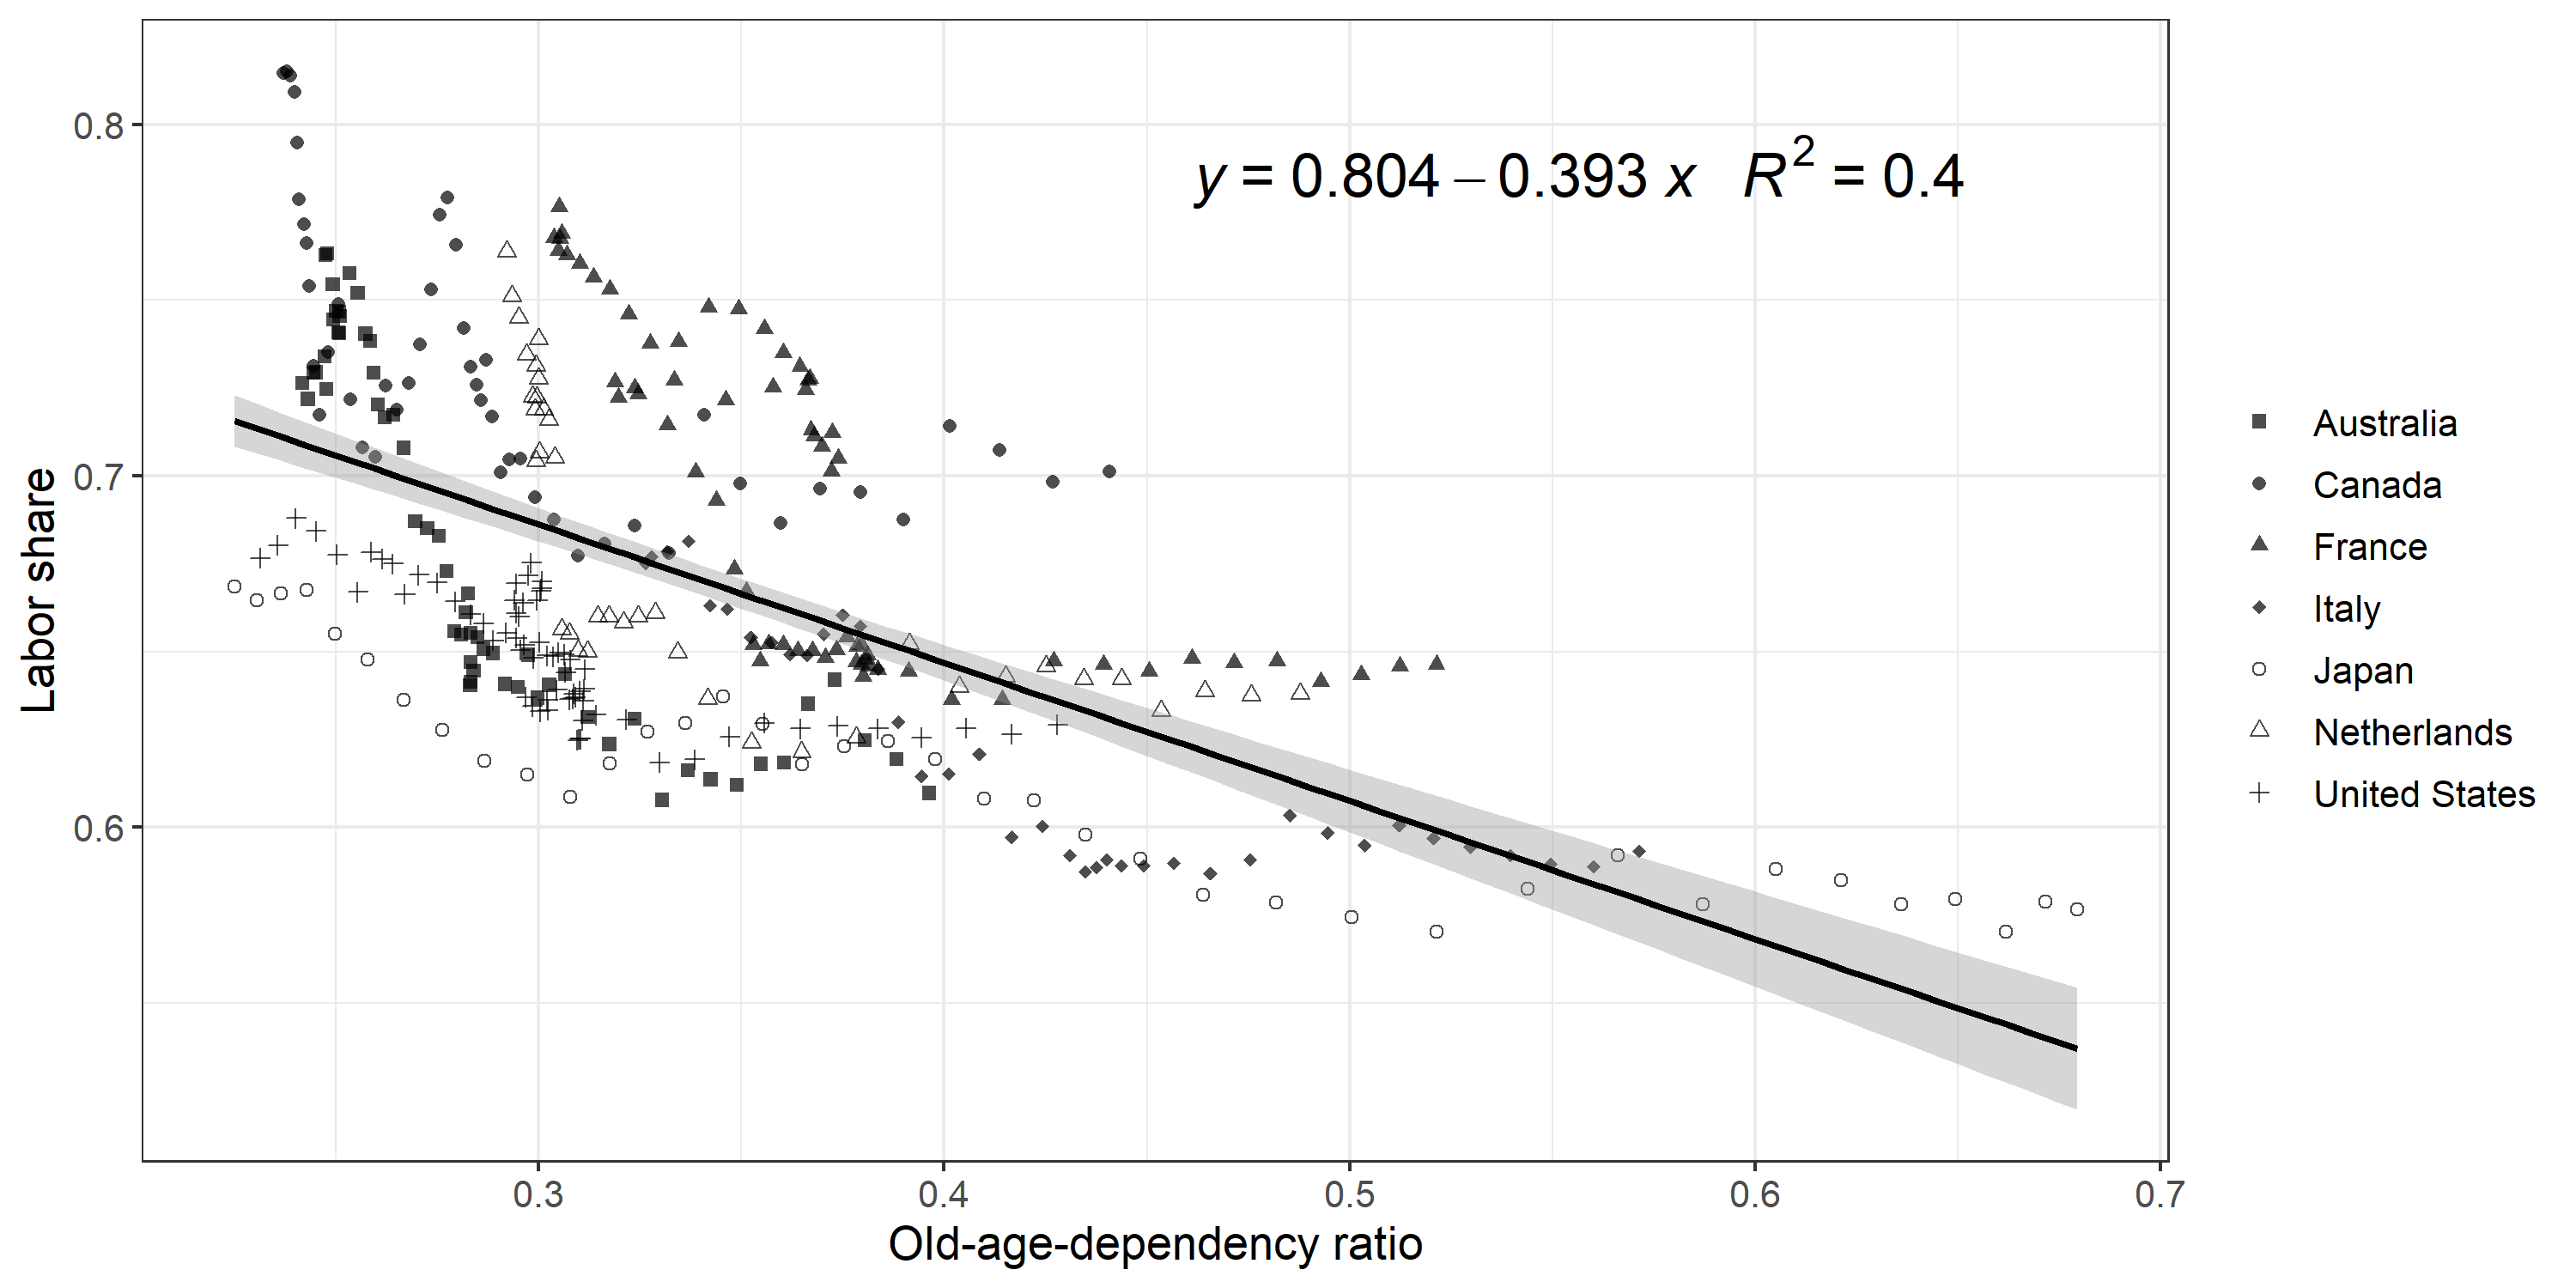
\includegraphics[width=\linewidth]{chap1/graphic/emp-lsdepcor.png}
	\vspace{-3em}
	\justify\singlespacing\footnotesize\textit{Notes:} The figure displays the negative correlation between the labor share and old-age-dependency ratio for several OECD countries. Labor share data are from the \href{https://www.rug.nl/ggdc/productivity/pwt/}{Penn World Table 10.0}. The old-age-dependency ratio is defined as the number of individuals above 60 over the number of those between 20 and 60. The ratio is computed with demographic data from the ``medium variant'' estimates from the \href{https://population.un.org/wpp/}{United Nations World Population Prospects 2017}.
\end{figure}
These data display a positive correlation, as the older the population the lower the labor share. 
Figure \ref{chap1-fig:emp-pubdepcor} shows cross-country correlations between the old-age-dependency ratio and the ratio between two public policy instruments, thus, providing empirical motivation also for linking public policy to the age structure of the population.\footnote{Looking also at the timing of labor market reforms---on employment protection legislation, public pension systems, non-employment benefits, and migration policies---in 14 OECD countries between 1986 and 2005, \citet{Pica2010Capital} shows that the number of reforms raising labor market flexibility has increased over time, hence, as the boomers' cohorts aged.}
\begin{figure}[!tb]
	\centering
	\caption{Public pension to unemployment spending ratio and old-age-dependency ratio}\label{chap1-fig:emp-pubdepcor}
	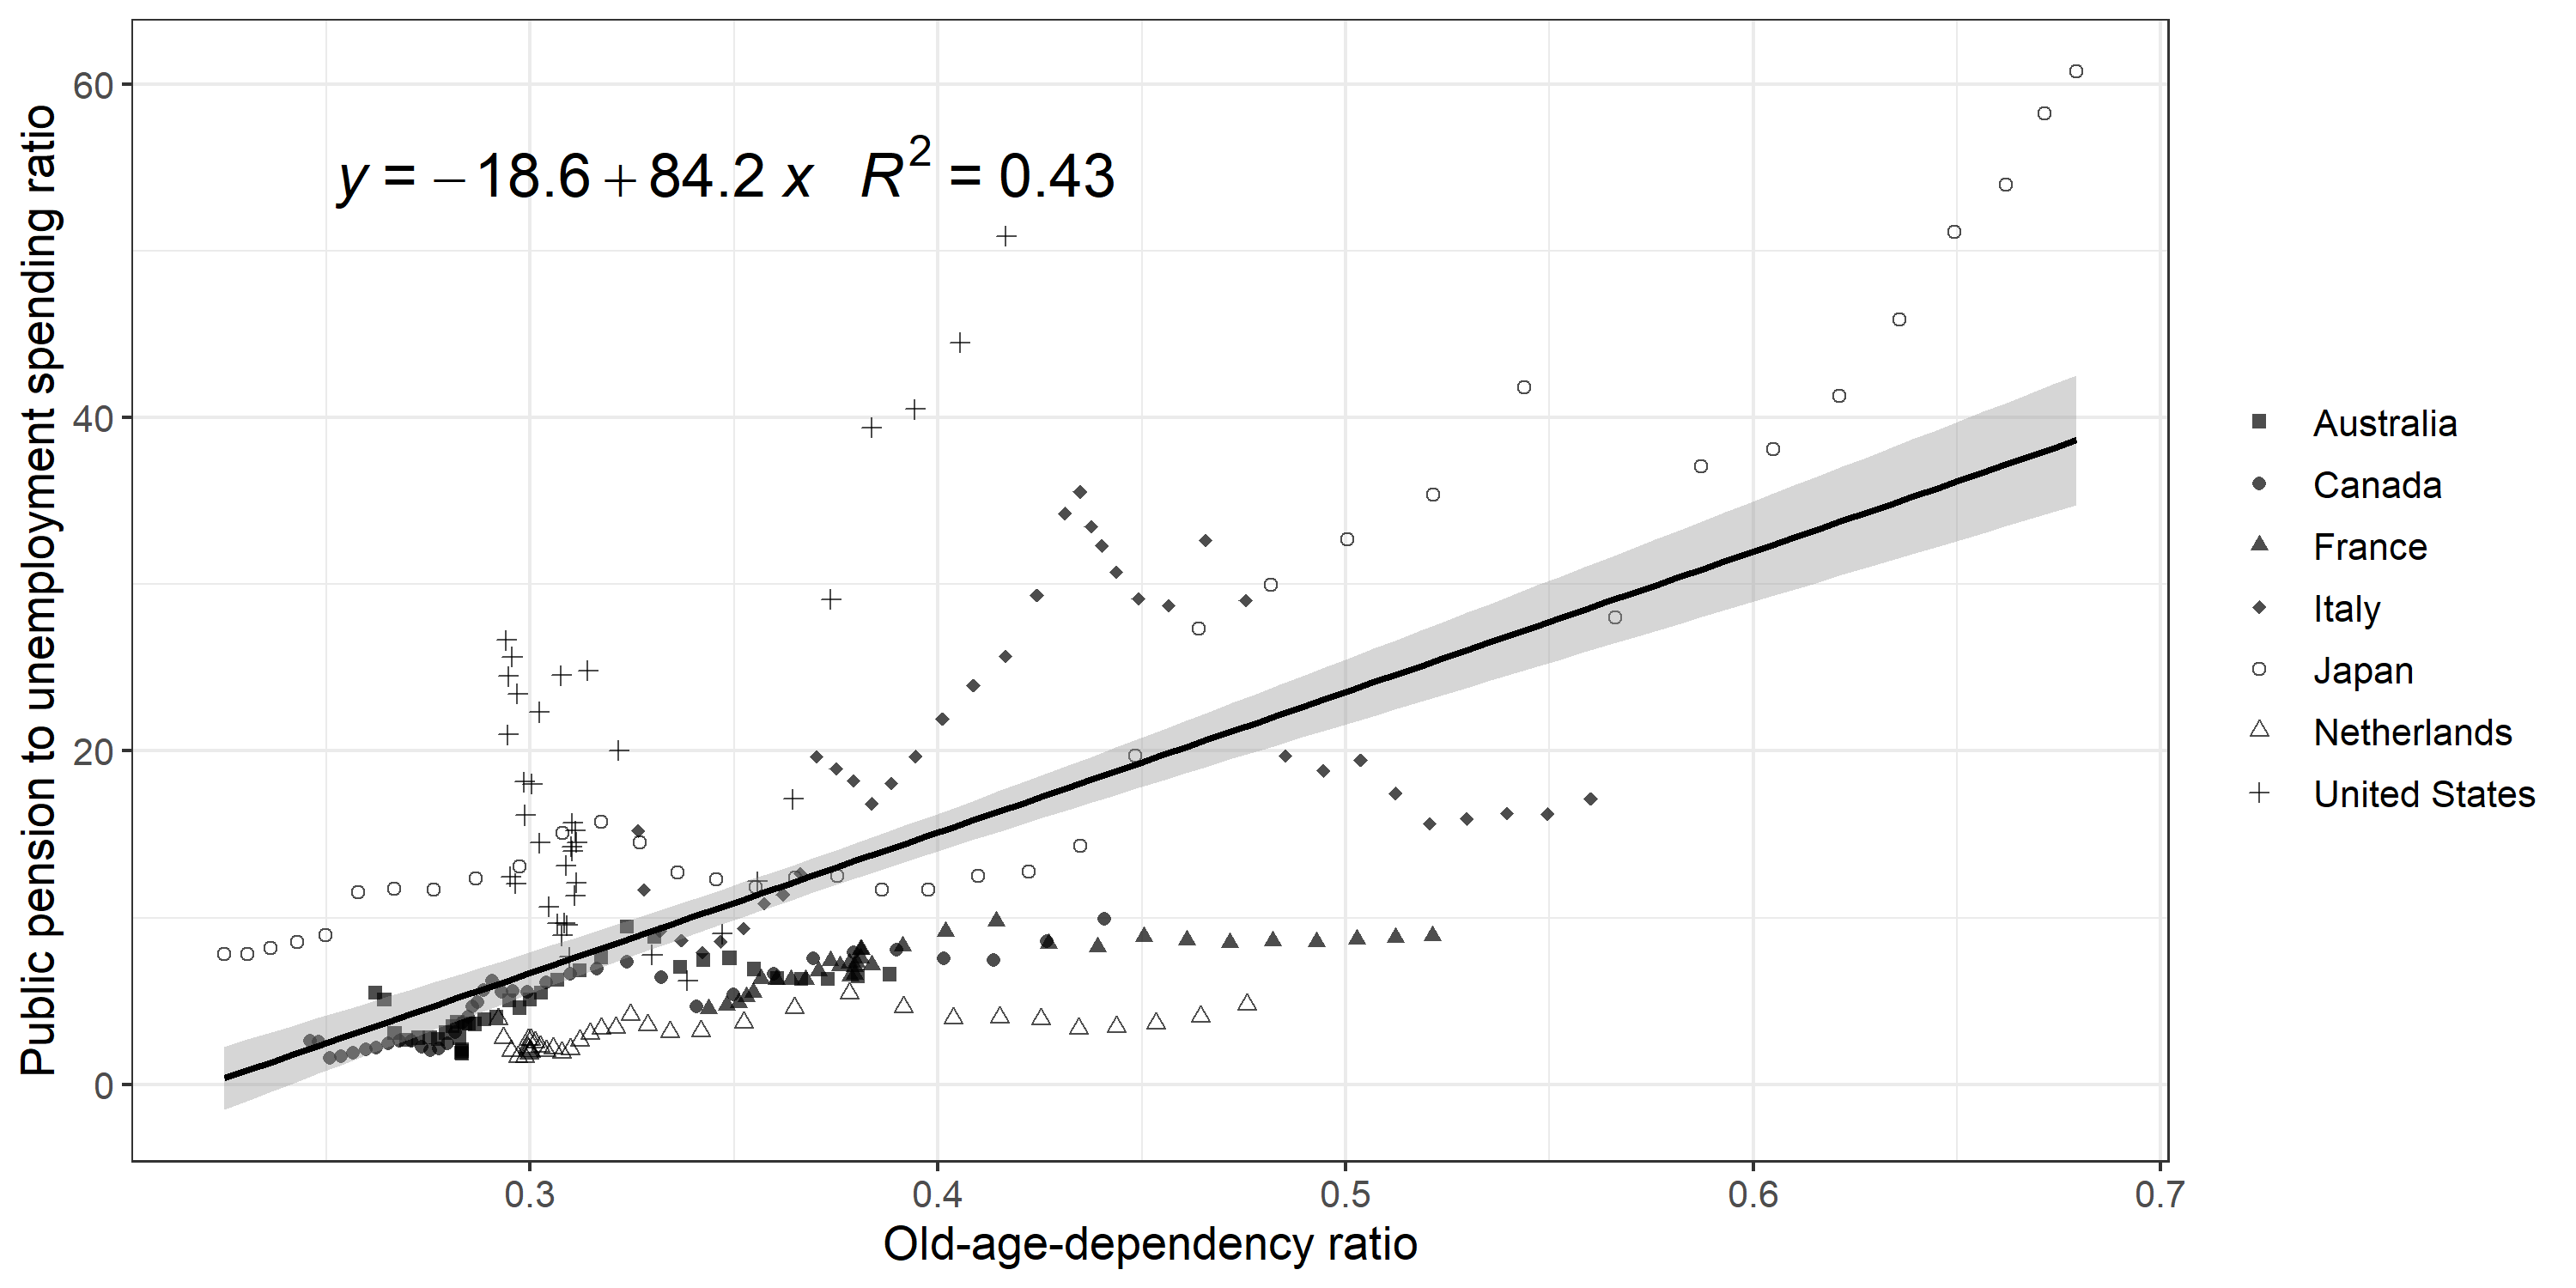
\includegraphics[width=\linewidth]{chap1/graphic/emp-pubdepcor.png}
	\vspace{-3em}
	\justify\singlespacing\footnotesize\textit{Notes:} The figure displays the positive correlation between the public pension to unemployment spending ratio and old-age-dependency ratio for several OECD countries. The public pension to unemployment spending ratio is computed using the total public unemployment spending and the total public pension spending (both as shares of GDP) from the OECD data. The old-age-dependency ratio is defined as the number of individuals above 60 over the number of those between 20 and 60. The ratio is computed with demographic data from the ``medium variant'' estimates from the \href{https://population.un.org/wpp/}{United Nations World Population Prospects 2017}.
\end{figure}
An increase in the old-age dependency ratio is associated with an increase in public pensions as a share of GDP relative to the share of unemployment spending. These data indicate that as the boomer cohorts age, public policy shifts in favor of old-age specific government spending.

% In this paper
In this paper, I argue that the observed shift away from labor toward capital is a response to changes in labor market institutions endogenously determined by the age structure of the population, a novel mechanism that this paper is the first to identify. Through this new \textit{policy-mechanism} effect, boomers drove the decline of the labor share when they were young and continue to drive it down nowadays as they retire. 

My argument is based on the idea that the boomers drive public policy choices because the size of their cohort gives them large political weight. When they are young, they change labor market institutions in their favor which allows them to bargain greater wages. To thwart workers' appropriation of rents, firms shift away from labor toward capital which decreases the labor share. Once the boomers become old and retire, we would expect a reversal of the labor share dynamics as pro-worker labor market institutions dwindle which increases employment. However, the consequent positive effect of employment on the labor share is offset by the capital accumulation fostered by extensive savings of the boomers when they were young, implying a further decline.

%% What I do
% Describe model
I develop a two-period OLG model with young and old households. Both vote to determine public policy while they have different income sources and opposite objectives. Old agents receive capital income and favor old-age specific government spending, whereas the youth receive wages and support unemployment benefits as they face unemployment risk. As a large cohort of boomers arrives, they use their political weight---through voting---to raise taxes and unemployment benefits. Both latter increase the outside option of workers in wage bargaining which allows them to bargain greater wages. The representative firm shifts away from labor toward capital. When labor and capital are gross substitutes, this leads to the decline of the labor share. Once the boomers retire, the political weight of the young declines and so does the unemployment benefit which fosters employment. However, the positive effect of employment on the labor share is offset by capital accumulation due to the extensive savings of young boomers which have been fostered by their higher bargained wages.

% Two mechanism
My framework suggests that demographic dynamics affect the labor share in two different ways. On the one hand, there is a direct \textit{factor-accumulation} effect operating through the labor supply and capital stock. A large generation expecting to live longer, such as the boomers, results in a higher labor supply when they are young and a larger capital stock---fostered by their savings---once they retire. On the other hand, there is an indirect \textit{policy-mechanism} effect reflecting the inter-generational conflict over public policy. A large generation has relatively more political weight---with respect to their elders and their youngsters---which allows it to shape the public budget allocation in its favor through voting.

% Consequences on the labor market
Both effects have consequences for the wage bargaining taking place in the labor market. The factor-accumulation effect encompasses two dynamics: a larger capital stock allows firms to substitute labor with capital which increases the capital-to-labor ratio; while a greater labor supply decreases wages which fosters employment, hence reducing the capital-to-labor ratio. Conversely, the consequence of the policy-mechanism effect is straightforward. When the political weight of the youth increases, so do unemployment benefits which raise workers' outside option. Workers bargain greater wages which undermines employment as firms substitute labor with capital, hence, raising the capital-to-labor ratio. The framework provides dynamics of the capital-per-worker with respect to demographic dynamics that \textit{do not depend on} the elasticity of substitution between capital and labor.

% Elasticity of substitution
The elasticity of substitution between capital and labor plays a crucial role in the model as it determines whether an increase in capital per worker raises or reduces the labor share. To calibrate the model, I estimate this elasticity, respectively, for France and the United States, and find, respectively, the values 1.21 and 1.27.\footnote{
I follow the specification of \citet{Klump2007Factor}, I estimate a single-equation estimation from the two first-order conditions of the profit maximization for a CES production function with biased technical change. Periods of the estimate correspond to 1950-2018 for France and 1950-2019 for the US. See section \ref{chap1-calibration} for the details.} 
Both elasticities being greater than one imply that capital and labor are gross substitutes. Thus, any increase of the capital per worker decreases the labor share, which corresponds to the stylized facts for several OECD countries (\citealt{Karabarbounis2014Global}). There is a substantive debate about the value of this elasticity in the literature. For the United States, many studies tend to find an elasticity between 0.4 and 0.6 (\citealt{Antras2004Aggregate}, \citealt{Chirinko2008Sigma}, \citealt{LeonLedesma2010Identifying}, i.a.). Nonetheless, \citet{Chirinko2017Substitution} recently show that this elasticity is much greater than one when considering income shares defined net of depreciation, which is in line with my theoretical framework. \citet{Rognlie2016Deciphering} also argues that accounting for depreciation is more relevant when dealing with income distribution issues. My estimate builds on the two latter arguments and supports recent estimates considered in the labor share literature.\footnote{
\citet{Caballero1998Jobless} use a capital-labor elasticity of substitution about 6 to simulate French data. \citet{Karabarbounis2014Global} use cross-sectional data on 50 countries between 1975 and 2012 to find a baseline estimate of the elasticity about 1.28. \citet{Piketty2015About} shows that the capital-income ratio and capital share tend to be positively correlated, thus, arguing that only an elasticity above one can reconcile this stylized fact with the one-sector standard model.}

% Quantitative analysis
I calibrate the model for France and the US starting in 1950. The model replicates labor share dynamics until the 2010s, along with those of the labor market. It also provides predictions of future dynamics. In France, the labor share is predicted to steadily decline from 64.7\% in 2020 to 60.4\% by 2100; while in the US, it is predicted to remain stable at 62.7\% until 2040 before declining to 58.8\% by 2100. From 2020 onward and until the end of the century, on average, about one percentage point of the labor income share will shift to capital income every 20 years.

% Counterfactual and decomposition
Counterfactual analysis shows that the policy-mechanism effect is as important as the factor-accumulation effect. In fact, the former partially offsets the latter effect when the boomers are young, hence, reducing the labor share. Once they retire, this newly-identified effect dominates. This pattern holds for both countries.

% Who are the winners
Lastly, I conclude by showing that boomers are the winners of the age-related conflict despite the decline of the labor share when they are young. They manage to compensate their labor income losses through redistribution due to their political weight. Thus, boomer cohorts have been better off in terms of income with respect to their elders and their youngsters.

%% Contributions
% 1/ Consequences of changes in the age structure of the population
My paper is related to several strands of the literature. First, I contribute to the growing literature on the consequences of demographic changes for the allocation between capital and labor income. 
\citet{Schmidt2013Demographic} show that an aging population leads to more savings, hence, more capital. When capital and labor are gross
substitutes, the accumulation of capital shrinks the labor share. 
I build on their mechanism--- which I define as the direct factor-accumulation effect---and introduce a new mechanism, namely, the indirect policy-mechanism effect. %, suggesting that labor market institutions are endogenous to these population dynamics.
\citet{Albis2021Demographic} empirically find that an exogenous change in the net population growth rate leads to a decline of the labor share; while an exogenous change in the net migration rate increases the labor share.
My paper provides a theoretical framework that can explain both patterns through the lens of the factor-accumulation and policy-mechanism effects.
Recent work has focused on changes in the labor share across industries. Notably, \citet{Acemoglu2022Demographics} argue that firms decide to rely more on automation technologies to replace middle-aged workers in manual production tasks as the latter become scarce due to population aging. They predict that the labor share should decline in industries that are intensive in those tasks.
My work provides an additional mechanism that relates firms' response to constraints in optimizing production factors owing to endogenous changes in labor market institutions fostered by demographic dynamics.

% 2/ Labor share determinants
Second, my work is related to the literature on the determinants of the labor share. These determinants have been widely studied and debated, ranging from globalization (\citealt{Jayadev2007Capital}, \citealt{Pica2010Capital}, \citealt{Young2018Globalization}, \citealt{Autor2020Fall}, i.a.) to capital-biased technical change (\citealt{Acemoglu2002Directed},  \citealt{Acemoglu2003Labor}, \citealt{Karabarbounis2014Global}, i.a.) and labor market institutions (\citealt{Blanchard1997Medium}, \citealt{Bentolila2003Explaining}, \citealt{Bental2010Declining}, i.a.). \citet{Caballero1998Jobless} argue that pro-labor income institutions are a burden to firms because they limit their ability to optimize inputs but also because they enable workers to obtain a high income share. As a response, firms shift away from labor toward capital through biased technical change. My paper looks upstream of the key mechanism in \citet{Caballero1998Jobless} and reproduces it without the need for biased technical change; rather I endogenize changes in labor market institutions which are determined by the age structure of the population. I hence show that demography is a key determinant of the labor share and suggest that it can be at the root of several explanations that the literature has measured (see, for instance, \citealt{Bergholt2021Decline}).

% 3/ Role of demography in shaping institutions and macro consequences
Third, the paper fits into the literature on the role of demography in shaping institutions and its consequences for macroeconomic outcomes (\citealt{Lee2010Macroeconomic}, \citealt{Aksoy2019Demographic}). Prior work focuses on the optimal retirement age for economic growth (\citealt{Futagami2001Population}, \citealt{Gonzalez-Eiras2012Ageing}, i.a.) or the sustainability of pension systems (\citealt{DelaCroix2013Aging}, \citealt{Dedry2017Aging}, i.a.). I contribute to this literature by providing insights on a key macroeconomic indicator that has never been considered by this debate, namely, the allocation of income between capital and labor.

% 4/ Boomers
Lastly, I contribute to the scarce literature on the consequences of cohort dynamics for aggregate labor-market dynamics (\citealt{Shimer1998Why}, \citealt{Ferraro2020Aging}). My results suggest that the boomers' generations are important drivers of the declining labor share in France and the US, a concept that has so far not been put forward.

% Plan
This paper is organized as follows. Section \ref{chap1-theory} describes the model starting with households, then presenting the labor market and public policy, to analyze the equilibrium. Section \ref{chap1-quantitative} provides the quantitative analysis. I start with the data, before calibrating the model. I present model predictions, compare the factor-accumulation and policy-mechanism effects, and discuss who are the winners of the age-related conflict. Section \ref{chap1-conclusion} concludes.
    
    \section{The model} \label{chap1-theory}
    %% Introduction of the model
% Household
I consider a two-period OLG model in which there are two types of households: young and old.
% Inter-generational conflict
The inter-generational conflict arises because young and old households have different preferences in terms of public policy; the former are in favor of higher unemployment benefits while the latter prefer more old-age specific government spending.

%%% Argue your choices (1 paragraph)
I model the inter-generational conflict over the public budget allocation with this trade-off between unemployment benefits and old-age specific government spending for two reasons.
%% 1/ Health expenditure are also for the young?
First, we can think about several types of government spending that are specific to old households. For instance, this can be interpreted as an old-age specific health expenditure or more broadly, public services such as residential care homes from which the elderly directly derive utility.\footnote{Although health spending is also for the young, it is correlated to age. \citet{Papanicolas2020Comparison} show that the US average per-capita health expenditure in 2015 is about three times larger for individuals above 65 with respect to those between 20 and 64. They also find an average ratio of about 3.14 for a sample of 8 OECD countries (excluding the US).}
%% 2/ Why don't you use a pension system?
Second, replacing this government spending with pensions would also be an alternative specification. Nonetheless, it would reduce the tractability of the model without any substantial gain in the analysis.\footnote{Pensions would introduce the policy instrument within the budget constraint of the old rather than directly in the utility function. From the point of view of the \textit{indirect policy mechanism}, the elderly would still desire more of this instrument. On the side of the \textit{direct factor-accumulation mechanism}, \citet{Schmidt2013Demographic} reach the same conclusions about the direct effect of aging on the labor share by considering an exogenous pension system. Moreover, additional assumptions would be required about the type of pension system, i.e. pay-as-you-go vs fully-funded pension system.}
To summarize, the model can be extended to other policy instruments for the old as long as they derive utility from it, either directly or through their income. The central point is to oppose young and old agents with different returns to policy instruments in utility terms.

Decisions within each period unfold as follows. First, young and old households vote to choose the tax rate, the unemployment benefit, and the old-age specific government spending, which defines the public policy equilibrium. 
Second, young households bargain over wages with the representative firm which determines the labor market equilibrium. 
Third, the uncertainty about the employment status of young households is resolved. 
Fourth, households choose their consumption and savings.
The vote and the bargaining jointly determine the equilibrium of the economy and, therefore, the labor share. I describe the model backward: starting with households, before presenting production and the labor market, and ending with the voting on public policy. Lastly, I analyze the equilibrium.

\subsection{Households}\label{chap1-households}

%% Demographic dynamics
The population consists of $N^y_t$ young and $N^o_t$ old individuals. Demographic dynamics are given by $N^y_t = n_t N^y_{t-1}$ where $n_t > 0$ is the gross rate of population growth, and $N^o_t = p_t N^y_{t-1}$ with $p_t \in \left(0,1\right]$ being the survival rate. The survival rate $p_t$ is an increasing function of life expectancy and a decreasing function of the retirement age.\footnote{In the model, agents are considered as old once they retire. If the life expectancy and the retirement age grow at the same rate, then the survival rate remains constant. For more details on the measurement of population aging, see \citet{Sanderson2007Perspective}; \citet{Sanderson2013Characteristics}; \citet{DAlbis2013Age}.} Both demographic parameters are exogenous and may vary over time. Their variations will generate population dynamics, and affect the old-age dependency ratio, $N^o_t/N^y_t = p_t/n_t$. 

%% Timing of the model and maximization program
Each cohort consists of a continuum of agents with identical preferences. Households have logarithmic utility functions and derive utility from consumption. Young households discount the future at factor $\alpha \in \left(0,1\right)$. They face an idiosyncratic longevity risk: with probability $p_{t+1}$ they survive and become old households in period $t+1$. Due to risk of death, the effective discount factor of young households equals $\alpha p_{t+1}$. 
Young households earn a disposable income $y_t$ that they allocate between consumption $c_{1,t}$ and savings $s_t$. 
Once old, they receive the net return of their savings $(1-\tau_{t+1}) s_t \hat{R}_{t+1}$, where $\tau_{t+1}$ is the tax rate and $\hat{R}_{t+1}$ the gross return on savings of a young household that survives to old age. I suppose a perfect annuities market where savings of young agents who die before becoming old are distributed among their surviving peers. Due to the perfect annuities market $\hat{R}_t = R_t/p_t$ where $R_t$ is the gross return on physical capital. Old households allocate all their capital income to consumption $c_{2,t+1}$ and also derive utility from old-age specific government spending $g_{t+1}$ which is a public good financed through taxes. This good can be interpreted as a variety of public expenditures---ranging from public provision of leisure activities to the pension of domestic helps---that increase the quality of life. Lastly, old households die at the end of period $t+1$.

% Maximization program
Maximizing expected utility, a household in period $t$ solves the following maximization problem:
\begin{align*}
	\max_{c_{1,t},~c_{2,t+1}}& U_t = \ln c_{1,t} + \alpha p_{t+1}\left( \ln c_{2,t+1} + \beta \ln g_{t+1} \right)\\
	\text{s.t.} ~~ &c_{1,t} + s_t = y_t,\\
	&c_{2,t+1} = (1-\tau_{t+1}) s_t \hat{R}_{t+1},
\end{align*}
% Define beta
where $\beta>0$ characterizes the preference for old-age specific government expenditure. The first-period disposable income $y_t$ depends on the employment situation of the household. Each young household faces an idiosyncratic unemployment risk with probability $u_t \in \left[0,1\right)$. The employment situation is known when choosing consumption and savings. An employed household earns a net wage $y_t^e= (1-\tau_t)w_t$ where $w_t$ is the wage rate, while an unemployed one gets the unemployment benefit $ y_t^u = b_t$ where $b_t$ are the unemployment benefits.

% FOC
Solving the household's maximization problem leads to the optimal consumption in both periods and savings in first period, which are
\begin{align}
	c_{1,t} &= \frac{1}{1+\alpha p_{t+1}} y_{t}, \label{chap1-eq:hhmaxc1}\\
	c_{2,t+1} &= \frac{\alpha p_{t+1}}{1+\alpha p_{t+1}}(1-\tau_{t+1})\hat{R}_{t+1}y_{t}, \label{chap1-eq:hhmaxc2}\\
	s_t &= \frac{\alpha p_{t+1}}{1+\alpha p_{t+1}} y_t. \label{chap1-eq:hhmaxs}
\end{align}
Since the utility function is logarithmic, savings are a constant proportion of disposable income. Aggregate savings in the economy are the weighted average of all disposable incomes of the young such that
\begin{equation}\label{chap1-eq:agg-saving}
	S_t = \frac{\alpha p_{t+1}}{1+\alpha p_{t+1}}\Big[(1-u_t)(1-\tau_t)w_t + u_t b_t\Big] N_t^y.
\end{equation}
I assume that capital fully depreciates between the two periods.\footnote{A period corresponds to half the lifetime of a generation, hence, I assume that capital is either depreciated or obsolete after such a long period.} Thus, equation \eqref{chap1-eq:agg-saving} determines the capital stock next period so that $K_{t+1} = S_t$. This assumption also implies that the gross return on physical capital is equal to the rental rate, i.e. $R_t = r_t$. 

\subsection{Labor market}\label{chap1-labor-market}

Consider a representative firm with a standard CES production function given by
\begin{equation}\label{chap1-eq:prod}
	Y_t = A\left[ \phi K_t^{\frac{\sigma - 1}{\sigma}} + (1-\phi) L_t^{\frac{\sigma - 1}{\sigma}}\right]^{\frac{\sigma}{\sigma-1}},
\end{equation}
where $K_t$ is the capital stock, $L_t$ labor, $\sigma$ the elasticity of substitution between capital and labor, $\phi$ the factor share parameter capturing the relative importance of inputs in production and $A$ a scale parameter. 
Rewriting the production function in per-worker terms, I have
\begin{equation}\label{chap1-eq:prod/L}
	\frac{Y_t}{L_t} = A\left(\phi k_t^{\frac{\sigma-1}{\sigma}} + 1-\phi\right)^{\frac{\sigma}{\sigma-1}},
\end{equation}
% Define k_t
where $k_t\equiv K_t/L_t$ is capital-per-worker.
The inverse labor demand function obtained from profit maximization is
\begin{equation}\label{chap1-eq:labor-demand}
	w_t = (1-\phi)A\left(\phi k_t^{\frac{\sigma-1}{\sigma}}+1-\phi\right)^{\frac{1}{\sigma-1}}.
\end{equation}

% Define labor share
% As long as the representative firm is on its labor demand curve, t
The labor share is defined as the ratio between the wage rate and output-per-worker, i.e. $\theta_t \equiv w_tL_t/Y_t$.
%
Using equations \eqref{chap1-eq:prod/L} and \eqref{chap1-eq:labor-demand}, the labor share is given by
\begin{equation}\label{chap1-eq:theta}
	\theta_t = \left(1+\frac{\phi}{1-\phi}k_t^{\frac{\sigma-1}{\sigma}}\right)^{-1}.
\end{equation}
%
Note that when the capital-labor elasticity of substitution equals unity, then the labor share is constant, i.e. $\theta_t=1-\phi$.
%
From equation \eqref{chap1-eq:theta}, we can also define the labor-to-capital income ratio as
\begin{equation}\label{chap1-eq:Theta}
	\Theta_t \equiv \frac{\theta_t}{1-\theta_t} = \frac{1-\phi}{\phi}k_t^{\frac{1-\sigma}{\sigma}}.
\end{equation}

The comparative statics of these expressions are straightforward. A higher capital-per-worker increases the wage and output per worker, i.e. $\partial w_t/\partial k_t > 0$ and $\partial (Y_t/L_t)/\partial k_t > 0$. However, the impact on the labor share depends on the elasticity of substitution between both factors, with $\partial \theta_t/\partial k_t \lessgtr 0$ if $\sigma \gtrless 1$. To have a negative relationship between the capital-per-worker and the labor share, both factors have to be gross substitutes, i.e. $\sigma > 1$. In such a case, any increase in capital per worker leads to a higher wage that is outweighed by the increase in output per worker. Thus, the labor share declines along with the labor-to-capital income ratio.

Young households bargain over the wage rate with the representative firm. The employer retains the prerogative to hire and fire as the labor market is a monopsony.\footnote{Possible extensions of the model would be to consider either a ``right-to-manage'' model \textit{à la} \citet{Nickell1983Unions} or an ``efficient contract'' model \textit{à la} \citet{McDonald1981Wage}. Both specifications introduce a representative union to bargain with the representative firm which strengthens the relative bargaining power of the workers by adding a distortion to the wage. In those settings, the bargaining power can be endogenous to public policy. Nonetheless, this goes far beyond the scope of the paper. With exogenous bargaining power, the right-to-manage specification leads to qualitatively equivalent results.} Consequently, the firm is always on its labor demand curve and equation \eqref{chap1-eq:labor-demand} holds. Since workers compete to get employed, they subsequently undercut their wages so that the wage rate is pinned down to their incentive constraint. The incentive constraint of workers is such that the net wage cannot be lower than their outside option, namely, the unemployment benefits, i.e. $(1-\tau_t)w_t \geq b_t$. Therefore, the labor market equilibrium wage---which implicitly characterizes the level of employment $L_t$---becomes
\begin{equation}\label{chap1-eq:labor-market}
    w_t = \frac{b_t}{1-\tau_t}.
\end{equation}

Using the labor demand function, as given by equation \eqref{chap1-eq:labor-demand}, I obtain $dL_t/db_t<0$ and $dL_t/d\tau_t<0, \forall \sigma$. When the unemployment benefit or the tax rate increase, so does the workers' outside option. As a result, workers bargain greater wages and the firm shifts away from labor toward capital to thwart workers' appropriation of the rents, i.e. the increase of labor costs. Therefore the model is able to replicate the partial equilibrium effect in \citet{Caballero1998Jobless} \textit{regardless of} the value of the elasticity of substitution between labor and capital.

\subsection{Public policy}\label{chap1-public-policy}

%% Describe government in the model (1 paragraph)
% Government revenue
The government taxes the labor income of the young and the returns to savings of the old at the same tax rate.\footnote{I consider a common tax rate to simplify the analysis. Young and old agents, both prefer a lower tax rate as it reduces their disposable income. By introducing different labor and capital income tax rates, I would have two sources of inter-generational conflict, adding complexity to the voting process but without providing additional insights.} The revenue generated from these taxes is allocated to unemployment benefits and old-age specific government spending. Therefore, the government budget constraint is $\tau_t\Big[ w_t(1-u_t)N^y_t + R_t S_{t-1} \Big] = b_t u_t N^y_t + g_t N^o_t$. Since the expression between square brackets corresponds to the total income in the economy $Y_t$, I rewrite the government budget constraint as
\begin{equation}\label{chap1-eq:gov-budget}
    \tau_t Y_t = b_t u_t N^y_t + g_t N^o_t.
\end{equation}

Everything else equal, both types of agents prefer lower taxes as they reduce their disposable income. The youth prefer a higher unemployment benefit since they face unemployment risk, while the elderly want more government spending because they derive utility from it.\footnote{Recall that households only care about the direct effects of public policy on their utility. Nonetheless, considering indirect effects---on the wage $w_t$ and interest rate $R_t$---would lead to the same conclusions concerning old households as any increase in unemployment benefits reduces the gross return on physical capital and therefore their income.} 

I make the key assumption that individuals make different policy choices when young and when old. Recent empirical evidence shows that people change their public spending preferences over their life cycle which reflects a form of age-related selfishness in public spending preferences. \citet{Sorensen2013Aging} shows that elderly people desire less spending in education while they support higher health expenditure and pensions. \citet{Busemeyer2009Attitudes} find sizable age-related differences in public policy preferences. Although these studies disagree on the magnitude of the conflict, they both show that such a conflict does exist.

% Explain the proba voting setup
I consider a probabilistic voting setup.\footnote{The alternative would be a median voter setup. However, the median voter setup would create two extreme regimes with one of them being a gerontocracy. It would also generate large swings in public policy if the median-voter switches from young to old or vice versa. Under probabilistic voting, the equilibrium policy platform is a continuous function of the old-age-dependency ratio.} With probabilistic voting, all agents vote for a policy platform $\psi_t = (\tau_t, b_t, g_t)$ represented by opportunistic candidates (or parties). Candidates try to maximize their probability of winning the election. They differ in their popularity and there is an idiosyncratic bias among voters for one candidate or the other. Candidates know about these biases. In equilibrium, all candidates choose the same policy platform $\psi_t^\star$ that maximizes the political objective function $W_t(\psi_t)$ defined below. See \citet{Lindbeck1987Balanced} for more details on the probabilistic-voting setup.

The youth vote before their employment status is revealed. There is no coordination between voting and wage bargaining. Therefore, households only care about the direct effects of public policy on their utility. They do not consider the indirect effects operating through unemployment, wages, and the accumulation of capital.
The maximization program that characterizes the public policy equilibrium is
\begin{equation*}
	\max_{\tau_t, b_t, g_t} W_t(\tau_t, b_t, g_t) = \eta_t \begingroup
    \underbrace{\bigg[ (1-u_t)\ln(1-\tau_t) + u_t \ln b_t\bigg]}_\text{Young indirect utility}\endgroup  + \begingroup
    \underbrace{\ln(1-\tau_t) + \beta \ln(g_t)}_\text{Old indirect utility}\endgroup
\end{equation*}
subject to the government budget constraint from equation \eqref{chap1-eq:gov-budget}, where 
\begin{equation}\label{chap1-eq:eta}
	\eta_t = \frac{n_t}{p_t}\omega(1+\alpha p_{t+1})
\end{equation}
is the \textit{political weight of the young}, and $\omega$ the relative ideological spread-out of the youth with respect to the elderly. The relative ideological spread-out is characterized by the ratio of the sensitivities of voting behavior to policy changes for each group. I assume this spread-out is constant over time.\footnote{This assumption can be interpreted in two ways: either both relative ideological spread-outs are time invariant or they vary in same proportions. It would be interesting to consider these spread-outs as endogenous or to make them cohort-specific. This goes beyond the scope of this paper.} See appendix \ref{chap1-probabilistic} for  more details about the probabilistic voting setup in this framework.

% Channel
The political weight is the key variable in the model because it is the channel through which the age structure affects public policy. It depends negatively on the old-age dependency ratio $p_t/n_t$. As expected, the older the population, the lower the political weight of the young in policy determination. It depends positively on the relative ideological spread-out $\omega$. The less ideological are the youth, the higher their political weight is because it is easier for the opportunistic candidates to get their votes with an appropriate public policy. As a consequence, candidates pay more attention to them. The political weight of the young is also increasing in the effective discount factor $\alpha p_{t+1}$. This term appears because the public policy at time $t$ also affects future income dynamics of the young generation.

Focusing on the interior solution of the maximization program, the first order conditions lead to the following public policy equilibrium:
\begin{align}
    b_t &= \frac{\eta_t}{1+\beta+\eta_t}\frac{Y_t}{N_t^y},\label{chap1-eq:unemp-spending}\\
    g_t &= \frac{\beta}{1+\beta+\eta_t}\frac{Y_t}{N_t^o},\label{chap1-eq:gov-spending}\\
    \tau_t &= \frac{\beta + u_t\eta_t}{1+\beta+\eta_t},\label{chap1-eq:tax-rate}
\end{align}
where equation \eqref{chap1-eq:unemp-spending} defines the unemployment benefits, equation \eqref{chap1-eq:gov-spending} the old-age specific government spending per old household, and equation \eqref{chap1-eq:tax-rate} gives the tax rate. 

Comparative statics are straightforward. The young generation desires higher taxation as long as the unemployment risk is large enough, i.e. $\partial \tau_t/\partial \eta_t > 0$ if and only if $u_t> \beta/(1+\beta)$. No matter the level of unemployment, they always prefer larger unemployment benefits, i.e. $\partial b_t/\partial \eta_t > 0$. Conversely, this generation desires less old-age specific government spending because they do not derive any utility from it yet, i.e. $\partial g_t/\partial \eta_t < 0$.\footnote{I do not consider any form of explicit altruism in the model. However, the parameter $\beta$ which is the preference for old-age specific spending captures a form of implicit altruism from young to their elders. The greater the parameter, the more individuals care about government spending once old.  Lastly, a form of explicit altruism from young to old generations would simply soften the age-related conflict without reversing its outcome.}

The aggregate net income of young households can be defined as
\begin{equation*}
    Y_t^y = \left[(1-u_t)(1-\tau_t)w_t + u_tb_t\right]N_t^y.
\end{equation*} Using equations \eqref{chap1-eq:labor-market} and \eqref{chap1-eq:unemp-spending}, I rewrite it as a share of the total income such that 
\begin{equation*}
    \frac{Y_t^y}{Y_t} = \frac{\eta_t}{1+\beta + \eta_t}.
\end{equation*}
For a given level of total income $Y_t$, the comparative statics indicate that when the political weight of the young rises, they increase their income share through more redistribution i.e. $\partial(Y_t^y/Y_t)/\partial\eta_t>0$. Conversely, the income share of the elderly shrinks when the political weight of the young increases, i.e. $\partial(Y_t^o/Y_t)/\partial\eta_t<0$. Furthermore, it is possible to express the after-tax income ratio between young and old households, as 
\begin{equation} \label{chap1-eq:after-tax-income-ratio}
	\frac{Y_t^y}{Y_t^o} = \eta_t.
\end{equation}
The greater is the political weight of the young, the greater their relative net income is, i.e. $\partial(Y_t^y/Y_t^o)/\partial\eta_t>0$.

\subsection{Equilibrium}\label{chap1-equilibrium}

Using equations \eqref{chap1-eq:unemp-spending} and \eqref{chap1-eq:tax-rate} from the public policy equilibrium along with equation \eqref{chap1-eq:labor-market} from the labor market equilibrium lead to the labor share at the equilibrium:
\begin{equation}\label{chap1-eq:equilibrium-theta}
    \theta_t = \frac{\eta_t(1-u_t)}{1+\eta_t(1-u_t)},
\end{equation}
where the political weight of the young $\eta_t$ is exogenous and given by demographic dynamics, while the unemployment rate $u_t$ is endogenous.
Using equation \eqref{chap1-eq:theta}, I can express the capital-per-worker at equilibrium as a function of exogenous variables, namely, 
\begin{equation}\label{chap1-eq:equilibrium-k}
    k_t^\star = \left(\frac{\phi}{1-\phi}\frac{K_t}{N_t^y}\eta_t\right)^\sigma,
\end{equation}
where the capital stock $K_t$ is given by the savings in previous period, whereas the labor supply $N_t^y$ and the political weight of the young are both given by the demographic dynamics. Thus, t here is a unique non-trivial equilibrium.

In equilibrium, the capital-per-worker is an increasing function of the political weight of the young $\eta_t$. The greater the political weight, the greater the unemployment benefits, hence, the bargained wage, thus, the lower the labor demand of the representative firm and the greater the capital-to-labor ratio as the firm relies more on capital than labor. Note that the intensity of the mechanism depends positively on the elasticity of substitution between capital and labor.

Since the capital stock is given by the savings in the previous period, i.e. $K_t = S_{t-1}$, the greater the savings of the previous generation, the larger the amount of capital available to the firm, hence, the larger the capital per worker. Conversely, the larger the young generation $N_t^y$, the larger the labor force, and therefore the lower the capital-to-labor ratio.

    
    \section{Quantitative analysis} \label{chap1-quantitative}
    % Objective of the quantitative analysis
This section presents the quantitative analysis of the model with three main objectives: to reproduce the labor share dynamics observed over the period 1950 to 2010, to provide model predictions after 2010, and to understand the transmission channels of demographic effects on the labor share. I compute model predictions for France and the United States. I focus on these two countries because they face important changes in the age structure of the population due to the emergence of the boomers' generation, while having sizeable differences in terms of labor market institutions and public policy.

% Follow the methodology of Gonzalez-Eiras and Niepelt
To simulate the model, I follow the methodology of \citet{Gonzalez-Eiras2012Ageing} which is standard in the literature to calibrate an OLG model. One period in the model is assumed to correspond to 40 years in the data. Thus, households are considered as young between 20 and 60 years of age and as old thereafter.\footnote{An implicit assumption of the model is that the retirement age is constant. The average French effective retirement age was 67.8 in 1970 and has declined to 59.3 in 2010. In the US it has gone from 68.4 to 65.6 over the same period (data from the \href{https://www.oecd.org/els/emp/average-effective-age-of-retirement.htm}{OECD Database, Ageing and Employment Policies - Statistics on average effective age of retirement}). I suppose, as an approximation, that agents retire at 60 years old to match the period lengths of the calibration. Such an assumption should not affect the voting outcome because almost-retired agents may anticipate their future situation once they vote. Nonetheless, a 5-year change remains moderate compared to the 40 years between two periods.}
I compute four sequences of model predictions with a period length of 40 years each. Periods of the first sequence correspond to 1950, 1990, 2030, 2070; for the second sequence to 1960, 2000, 2040, 2080; for the third sequence to 1970, 2010, 2050, 2090; and for the fourth sequence to 1980, 2020, 2060, 2100. When I report time-series predictions, I list these four sequences in a single time series. Thus, there are always eight generations living simultaneously, four of them being young and the four others old. Every 10 years, a new generation is born and an old one dies.

\subsection{Data}\label{chap1-data}

\textbf{Demography.} I use demographic data from the \href{https://population.un.org/wpp/}{United Nations World Population Prospects 2017}.%
\footnote{Demographic data from 1950 to 2010 come from the \href{https://population.un.org/wpp/}{United Nations World Population Prospects 2017}. For future dynamics, I rely on the ``medium variant'' estimates from the United Nations. Demographic data before 1950 are from \href{http://www.populstat.info}{http://www.populstat.info}. Due to data limitations, the expected survival rate $p_{t+1}$ is not available after 2060. Thus, I suppose that $p_{t+1}$ grows at its observed average growth rate until 2060, for each country, hence, 4.921\% for France and 4.137\% for the United States. Nevertheless, I limit my analysis to 4 periods (hence 2100) due to the large degree of uncertainty thereafter.}
I start by computing the old-age dependency ratio from the data as the number of old individuals divided by the number of young ones. Then, I compute the population growth rate using the ratio between the number of young individuals relative to the number of young people in the previous period of the sequence, i.e. $n_t = N_t^y/N_{t-1}^y$. Lastly, the survival rate verifies the identity and equals the product of the old-age-dependency ratio and the population growth, i.e. $p_t \equiv N_t^o/N_t^y\times n_t$. Figure \ref{chap1-fig:demo} plots demographic dynamics for France and the United States and indicates that both countries face the same demographic context.
\begin{figure}[!tb]
	\centering
	\caption{Demographic dynamics}\label{chap1-fig:demo}
	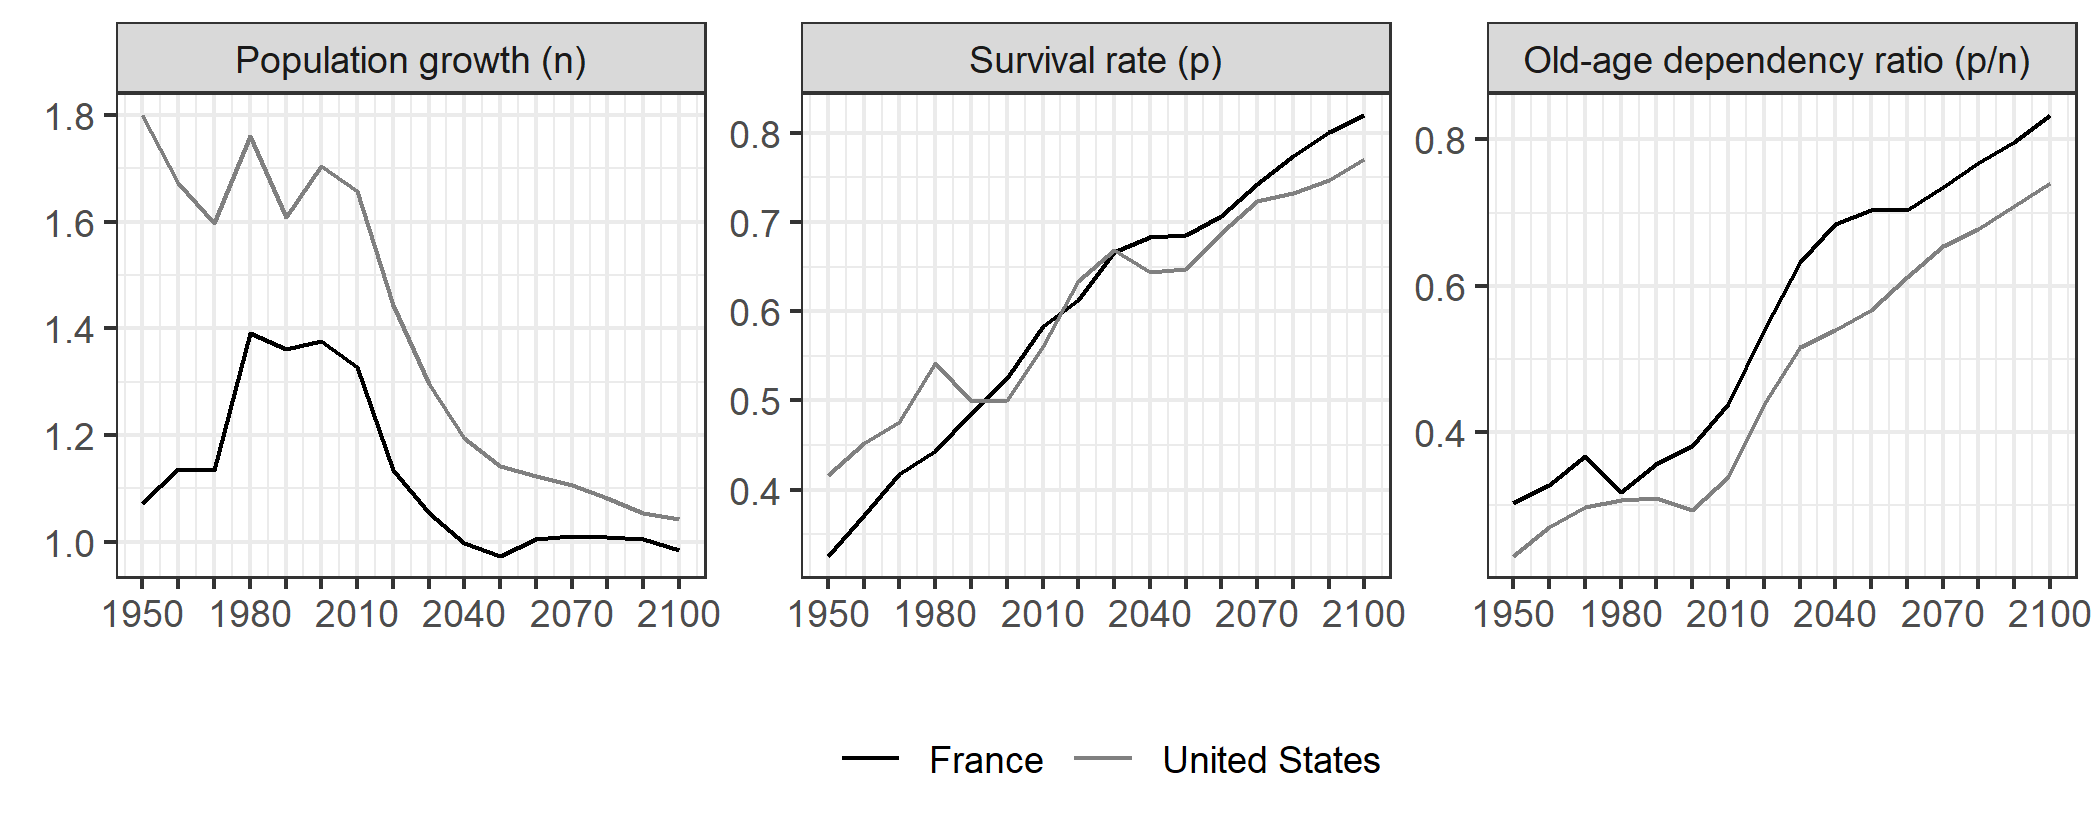
\includegraphics[width=\linewidth]{chap1/graphic/quant-demo.png}
	\vspace{-3em}
	\justify\singlespacing\footnotesize\textit{Notes:} The figure displays, for each country every 10 years, the population growth rate, the survival rate and the old-age dependency ratio. Data correspond to the ``medium variant'' estimates from the  \href{https://population.un.org/wpp/}{United Nations World Population Prospects 2017}.
\end{figure}
I distinguish three eras in terms of dynamics that correspond to the life cycle of the boomers' generation: when the boomers are young between 1970 and 2010; when they retire; and thereafter once they disappeared. Until 2010, the old-age dependency ratio remains roughly stable due to the massive entry of the boomers into the labor force that offsets the rise in the survival rate due to increasing life expectancy. Thereafter, as the boomer generation retires, the survival rate continues to grow and population growth declines. As a consequence, the old-age dependency ratio explodes.

\textbf{Labor share.} I use labor share data from the \href{https://www.rug.nl/ggdc/productivity/pwt/}{Penn World Table 10.0} (PWT); see \citet{Feenstra2015Next} for more details on these data. In this dataset, the labor share $\theta_t$ corresponds to the share of labor compensation in GDP. As argued by \citet{Gollin2002Getting}, the measurement of the labor share is influenced by the adjustment method to take into account self-employed income. In the theoretical framework, workers are young individuals and supply only labor. In line with the model, I consider self-employed income as labor compensation.

\textbf{Capital stock.} I use the capital stock at constant 2011 national prices from the PWT for the capital stock $K_t$. To disentangle the effect of changes in the number of hours worked, I adjust both variables by the average annual hours worked by persons engaged from the same data source.

\textbf{Labor and unemployment.} I also use the number of persons in employment from the PWT. In the model, labor supply is inelastic and there is no distinction between unemployed and inactive individuals. The unemployed, in terms of the model specification, correspond to all agents that do not work. However, in high-income countries such as France and the United States, inactive people also benefit from redistribution through transfer payments. Therefore, I treat them as unemployed and the redistribution is captured through unemployment benefit $b_t$ in the model. I compute the unemployment rate such that $u_t = 1 - emp_t/N^{15-64}_t$, where $emp_t$ is the number of persons in employment and $N_t^{15-64}$ is the working-age population.\footnote{I consider the whole working-age population instead of the young population. Due to the demographic specification of the model, young agents correspond to those between 20 and 60 years old. Data on the number of persons engaged per age group are not available in PWT. Therefore, taking only $N^y_t$ as denominator would bias downward the unemployment rate. % Results are robust to different specifications of the unemployment rate.
Although there are other sources of population data, I rely on the PWT to have consistency using the same data source for input factors and output.}
Then, I compute labor according to the identity $L_t\equiv(1-u_t)N_t^y$.

\textbf{Public policy variables.} I use the government revenue as a share of GDP from the \href{https://www.oecd.org/tax/tax-policy/tax-database/}{OECD Tax Database} to proxy the tax rate $\tau_t$, these data are not available before 1970. I use the pension spending expressed in percentage of GDP as a measure of the old-age specific government spending, i.e. $g_tN^o_t/Y_t$, as it is likely to be positively correlated with. Lastly, I consider the public unemployment spending expressed in percentage of GDP for the share of total unemployment benefits, i.e. $b_tu_tN^y_t/Y_t$. Both latter variables are from the OECD data.

\textbf{Normalization.} 
I normalize the capital-labor ratio $k_t$ and the young population $N_t^y$ to their 1950 values. $L_t$ is computed such that the unemployment rate $u_t$ matches the one derived for 1950 and $K_t$ satisfies the identity $k_t \equiv K_t/L_t$.

\subsection{Calibration}\label{chap1-calibration}

% Calibration
Once stock variables are normalized, I calibrate the parameters of the model $\{ \alpha,$ $\phi,$ $\sigma,$ $\omega,$ $\beta,$ $A \}$. Table \ref{chap1-tab:quant-param} summarizes parameters for both countries.
\begin{table}[!tb]
    \centering
    \begin{threeparttable}
        \caption{Parameters} \label{chap1-tab:quant-param}
        
\begin{tabular}{llrrl}
\toprule
\textbf{} & \textbf{Parameter} & \textbf{France} & \textbf{US} & \textbf{Target}\\
\midrule
$\alpha$ & Discount rate & 0.669 & 0.669 & Set to $0.99^{40}$\\
$\phi$ & Capital share in 1950 & 0.232 & 0.323 & $1-\theta_{1950}$\\
$\sigma$ & Capital-labor elasticity of substitution & 1.206 & 1.270 & Estimation\\
$\omega$ & Relative ideological spread-out & 1.103 & 0.622 & $k_{1970}$\\
$\beta$ & Preference for old-age specific gov. spending & 0.570 & 0.002 & $\tau_{1970}$\\
$A$ & Scale parameter of the production function & 127.782 & 18.430 & $\theta_{1990}$\\
\bottomrule
\end{tabular}

        \begin{tablenotes}[flushleft]
            \footnotesize\item \textit{Notes}: The table reports the parameters and the targets from the calibration of the model for France and the United States. The discount rate is set to 0.99 on annual basis. The capital share in 1950 matches the labor share in the same year.
            The capital-labor elasticity of substitution is obtained with a single-equation estimation from the two first-order conditions of the profit maximization with normalized CES production function.
            The relative ideological spread-out matches the capital-labor ratio in 1970, the preference for old-age specific government spending matches the tax rate in 1970, and the scale parameter of the production function matches the labor share in 1990.
        \end{tablenotes}
    \end{threeparttable}
\end{table}
I set the discount rate $\alpha$ at 0.669, i.e. 0.99 on annual basis. 
The parameter $\phi$ corresponds to the capital share in 1950 and is derived from the labor share in the same year. 

The main parameter of the model is the elasticity of substitution between capital and labor, i.e. $\sigma$. I follow the specification of \citet{Klump2007Factor} for a CES production function with biased technical change. % \textit{à la} \citet{David1965Biased}. 
I estimate $\sigma$ with a single-equation estimation from the two first-order conditions of the profit maximization, namely,
\begin{equation} \label{chap1-eq:est-sigma}
	\ln \Theta_t = \gamma_0 + \gamma_1 \ln (k_t/k_0) + \gamma_2\left(t-t_0\right),
\end{equation}
where $\gamma_0$ is the intercept, $\gamma_1\equiv(1-\sigma)/\sigma$ encompasses the elasticity of substitution between both factors, and $\gamma_2$ captures the overall bias in technical change.

Table \ref{chap1-tab:sigma-estimate-short} summarizes the coefficients and provides the estimated elasticity for both countries.
\begin{table}[!tb]
    \centering
    \caption{Estimation of the capital-labor elasticity of substitution} \label{chap1-tab:sigma-estimate-short}
    \begin{threeparttable}
        \setlength{\tabcolsep}{12pt}
        \begin{tabular}{l D{.}{.}{2.6} D{.}{.}{2.6} D{.}{.}{2.6} D{.}{.}{2.6}}
\toprule
 & \multicolumn{4}{c}{Linear regression - OLS} \\
\cmidrule(lr){2-5}
 & \multicolumn{2}{c}{France} & \multicolumn{2}{c}{United States} \\
\cmidrule(lr){2-3}\cmidrule(lr){4-5}
 & \multicolumn{1}{c}{(1)} & \multicolumn{1}{c}{(2)} & \multicolumn{1}{c}{(1)} & \multicolumn{1}{c}{(2)} \\
\midrule
$\gamma_1$ & 1.233^{***}  & 1.214^{***}  & 0.752^{***}  & 0.762^{***}  \\
           & (0.020)      & (0.019)      & (0.012)      & (0.014)      \\
$\gamma_2$ & -0.318^{***} & -0.171^{***} & -0.213^{***} & -0.363^{***} \\
           & (0.014)      & (0.043)      & (0.017)      & (0.101)      \\
$\gamma_3$ &              & -0.005^{***} &              & 0.002        \\
           &              & (0.001)      &              & (0.002)      \\
\midrule
$\sigma$ & \multicolumn{1}{c}{1.466} & \multicolumn{1}{c}{1.206} & \multicolumn{1}{c}{1.270} & \multicolumn{1}{c}{1.571} \\
\midrule
R$^2$ & \multicolumn{1}{c}{0.891} & \multicolumn{1}{c}{0.908} & \multicolumn{1}{c}{0.703} & \multicolumn{1}{c}{0.713}\\
Adj. R$^2$ & \multicolumn{1}{c}{0.889} & \multicolumn{1}{c}{0.906} & \multicolumn{1}{c}{0.699} & \multicolumn{1}{c}{0.704}\\
Num. obs. & \multicolumn{1}{c}{69} & \multicolumn{1}{c}{69} & \multicolumn{1}{c}{70} & \multicolumn{1}{c}{70}\\
\bottomrule
\end{tabular}

        \begin{tablenotes}[flushleft]
            \footnotesize{\item\textit{Notes}: $^{***}p<0.01$; $^{**}p<0.05$; $^{*}p<0.1$. Standard errors between parentheses. The labor-to-capital income ratio (in log) is the dependent variable. The periods of the estimate correspond to 1950-2018 for France and 1950-2019 for the US. Single-equation estimation from the two first-order conditions of the profit maximization for a CES production function with biased technical change. Coefficients are as follows. $\gamma_0$ is the intercept, $\gamma_1\equiv(1-\sigma)/\sigma$ encompasses the elasticity of substitution between capital and labor, and $\gamma_2$ captures the overall bias in technical change.}
        \end{tablenotes}
    \end{threeparttable}
\end{table}
For France, the specification in column (2) that controls for the bias of technical change is the preferred one. Since $\gamma_3$ is negative and significant it means that the technical change is biased toward capital.
For the US, I consider the first specification as $\gamma_3$ is not significant in column (2). Note that the coefficients from which I derive the elasticity, i.e. $\gamma_2$, are significantly negative, implying that $\sigma$ is significantly greater than one.
I hence obtain an elasticity of 1.206 for France and 1.270 for the United States.
Therefore, both input factors are gross substitutes. These values are in line with recent estimates in the literature on the labor share such as \citet{Karabarbounis2014Global} who use cross-sectional data on 50 countries over the period 1975-2012 to find an elasticity greater than 1, with an average of 1.28 in their baseline estimates.\footnote{\citet{Caballero1998Jobless} use a relatively high value of the capital-labor elasticity of substitution, about 6.00, to simulate French data.}

% 3 remaining parameter => match moments
To calibrate the three remaining parameters, I match three moments in the data. 
% OMEGA
The relative ideological spread-out $\omega$ is set to match the capital-labor ratio $k_t$ in 1970 using equation \eqref{chap1-eq:equilibrium-k}.
The parameter being greater in France than in the US, it suggests that young people have inherently more political weight in France compared to the US.
% BETA
The preference for old-age specific government spending $\beta$ is set to match the tax rate $\tau_t$ in 1970, from the data, using equation \eqref{chap1-eq:tax-rate}.
% beta FR > beta US
As expected, the preference for old-age specific government expenditure---relative to private consumption---is greater in France than in the United States.
% A (scale parameter)
Lastly, the scale parameter of the production function $A$ is set to match the average labor share between 1988 and 1992.

\subsection{Model predictions}\label{chap1-model_pred}

I simulate the model using the parameters values above. For the remaining of the paper, I refer to this simulation as the benchmark simulation. Figure \ref{chap1-fig:quant-bench-ls} displays the labor shares predicted by the model.
\begin{figure}[!tb]
	\centering
	\caption{Model predictions of the labor share} \label{chap1-fig:quant-bench-ls}
	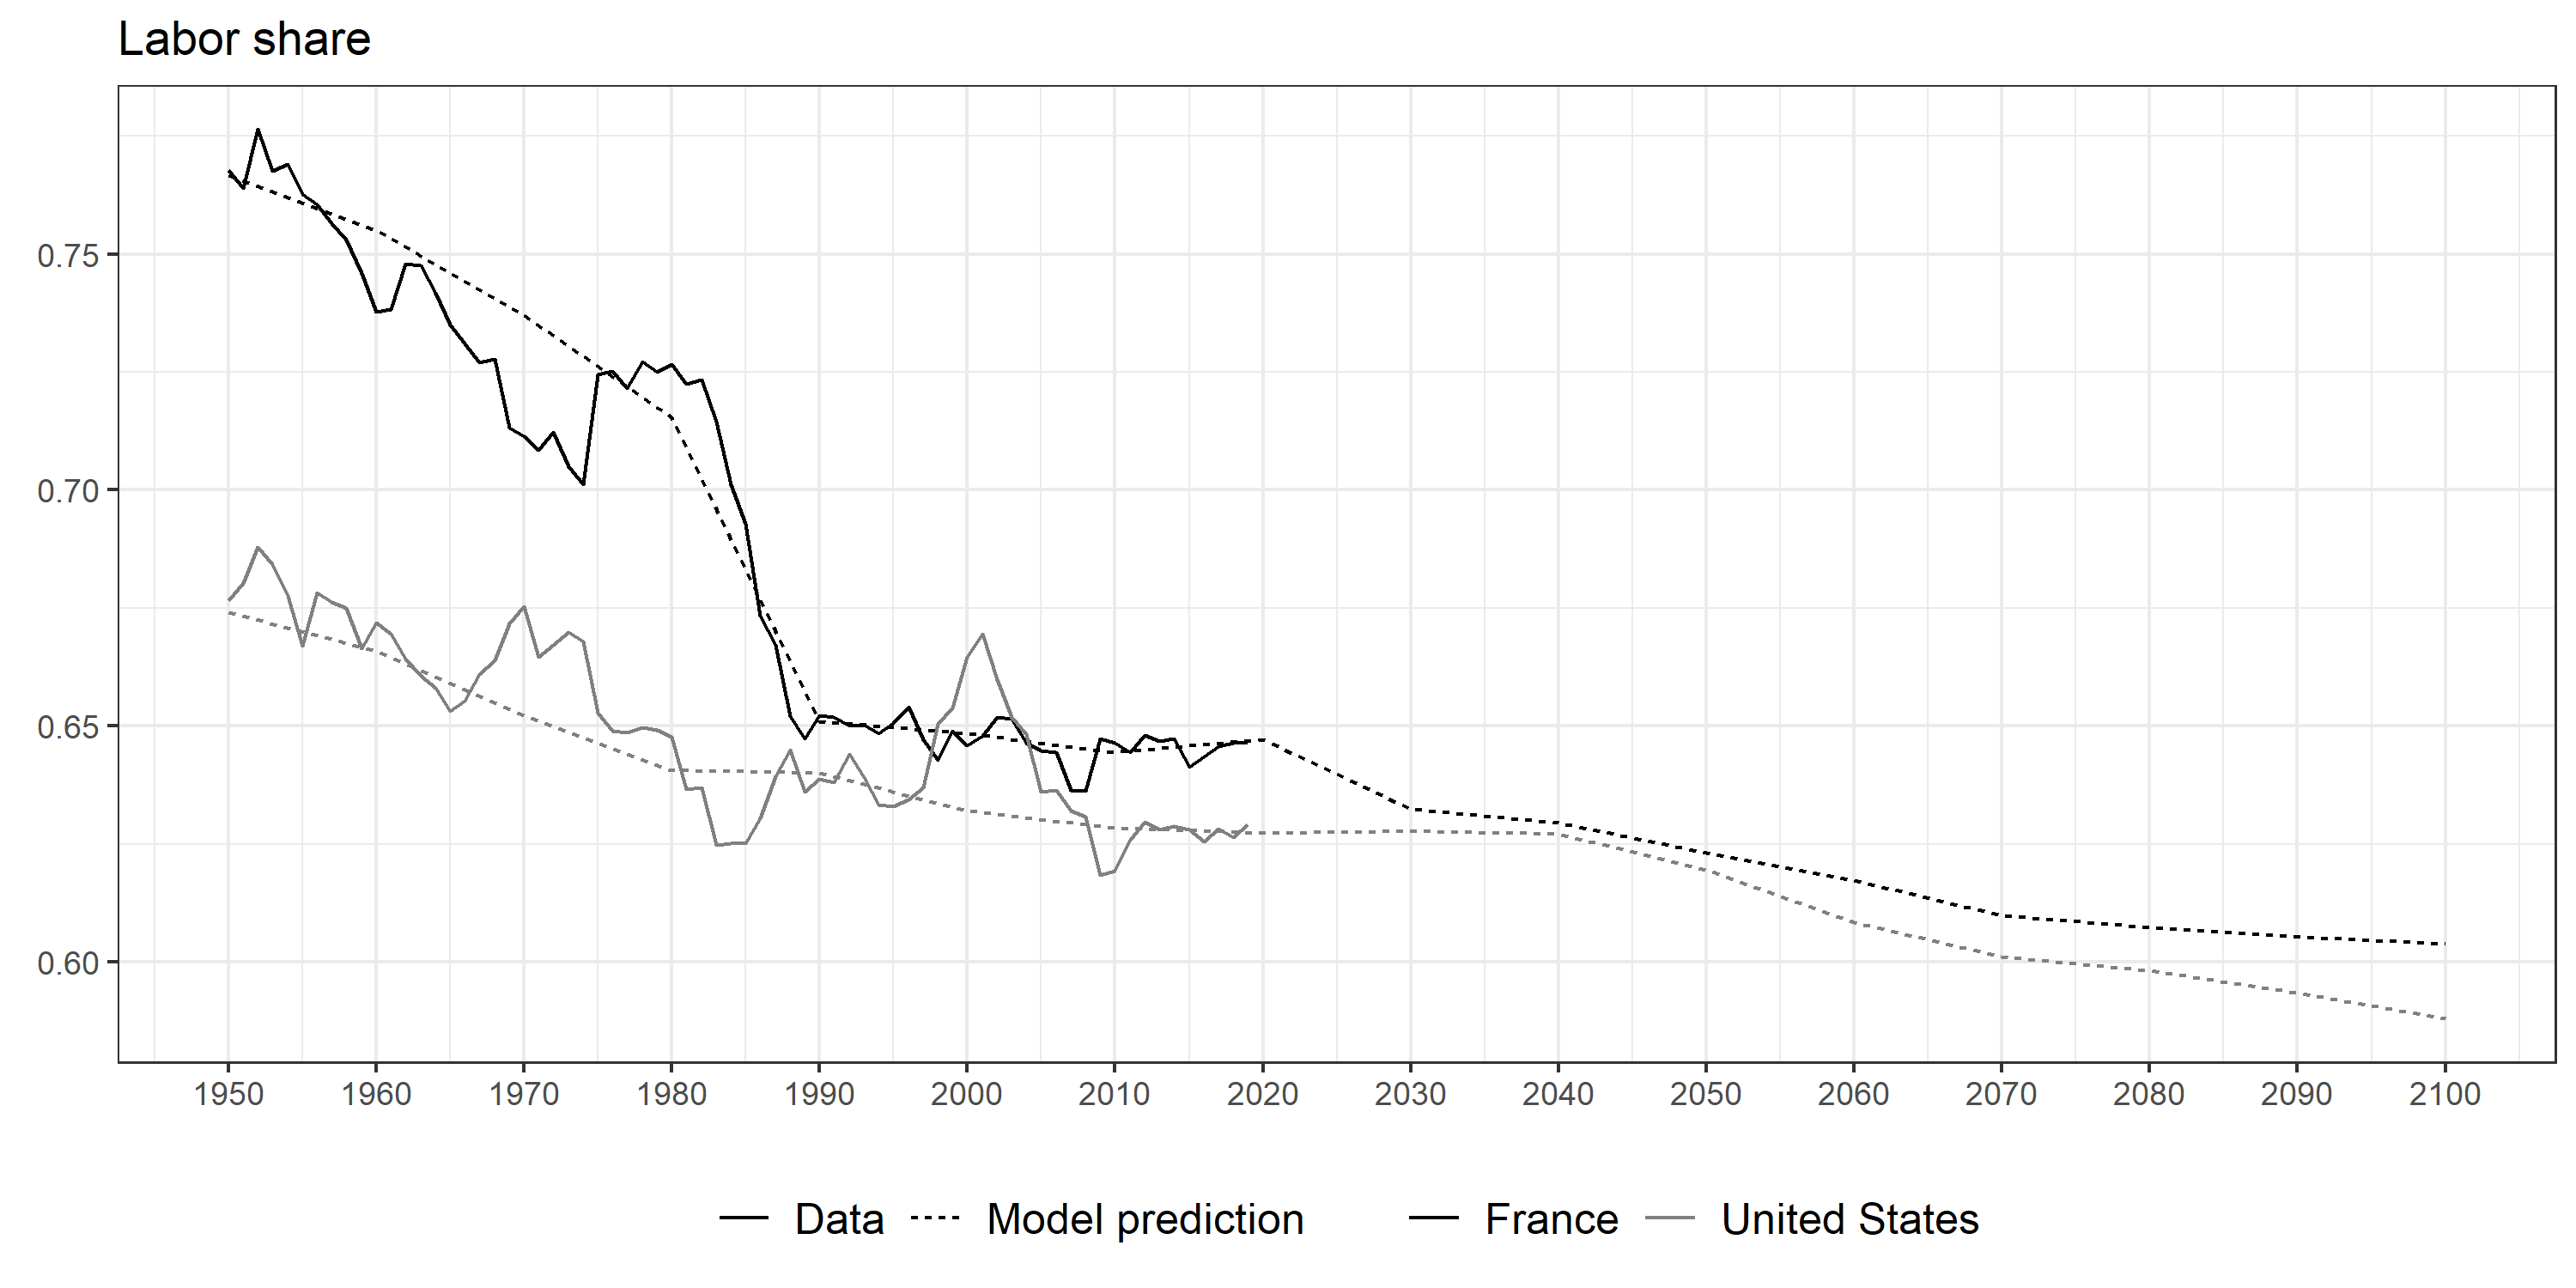
\includegraphics[width=1\linewidth]{chap1/graphic/quant-bench-ls.png}
	\vspace{-3em}
	\justify\singlespacing\footnotesize\textit{Notes:} The figure shows the labor share predictions of the model (dashed lines) and the labor share in the data (solid lines) from 1950 to 2100 for France and the US.
	Labor share data are from the \href{https://www.rug.nl/ggdc/productivity/pwt/}{Penn World Table 10.1} with self-employed income as labor compensation.
\end{figure}
The model reproduces the global trend in the data for both countries until 2020. For the US, the model underestimates the labor share around 2000. However, it captures the overall trend of the labor share over the period.
For France, model predictions are more accurate and reproduce the data since 1950. Looking at the model's predictions after 2020, the labor share should decline until the end of the century in both countries. I discuss the dynamics of variables---in the public policy equilibrium and in the labor market equilibrium---over the three periods: when the boomers are young (1970-2010), when they are retired (2010-2050), and afterward (2050-2100).

%% Other economic variables before 2010
\textbf{The young boomers (1970-2010).} 
Figure \ref{chap1-fig:quant-bench-dev7010-pub} displays the dynamics of public policy variables, expressed in percentage deviation from their 1970's value.
\begin{figure}[!tb]
	\centering
	\caption{Public policy dynamics over the 1970-2010 period} \label{chap1-fig:quant-bench-dev7010-pub}
	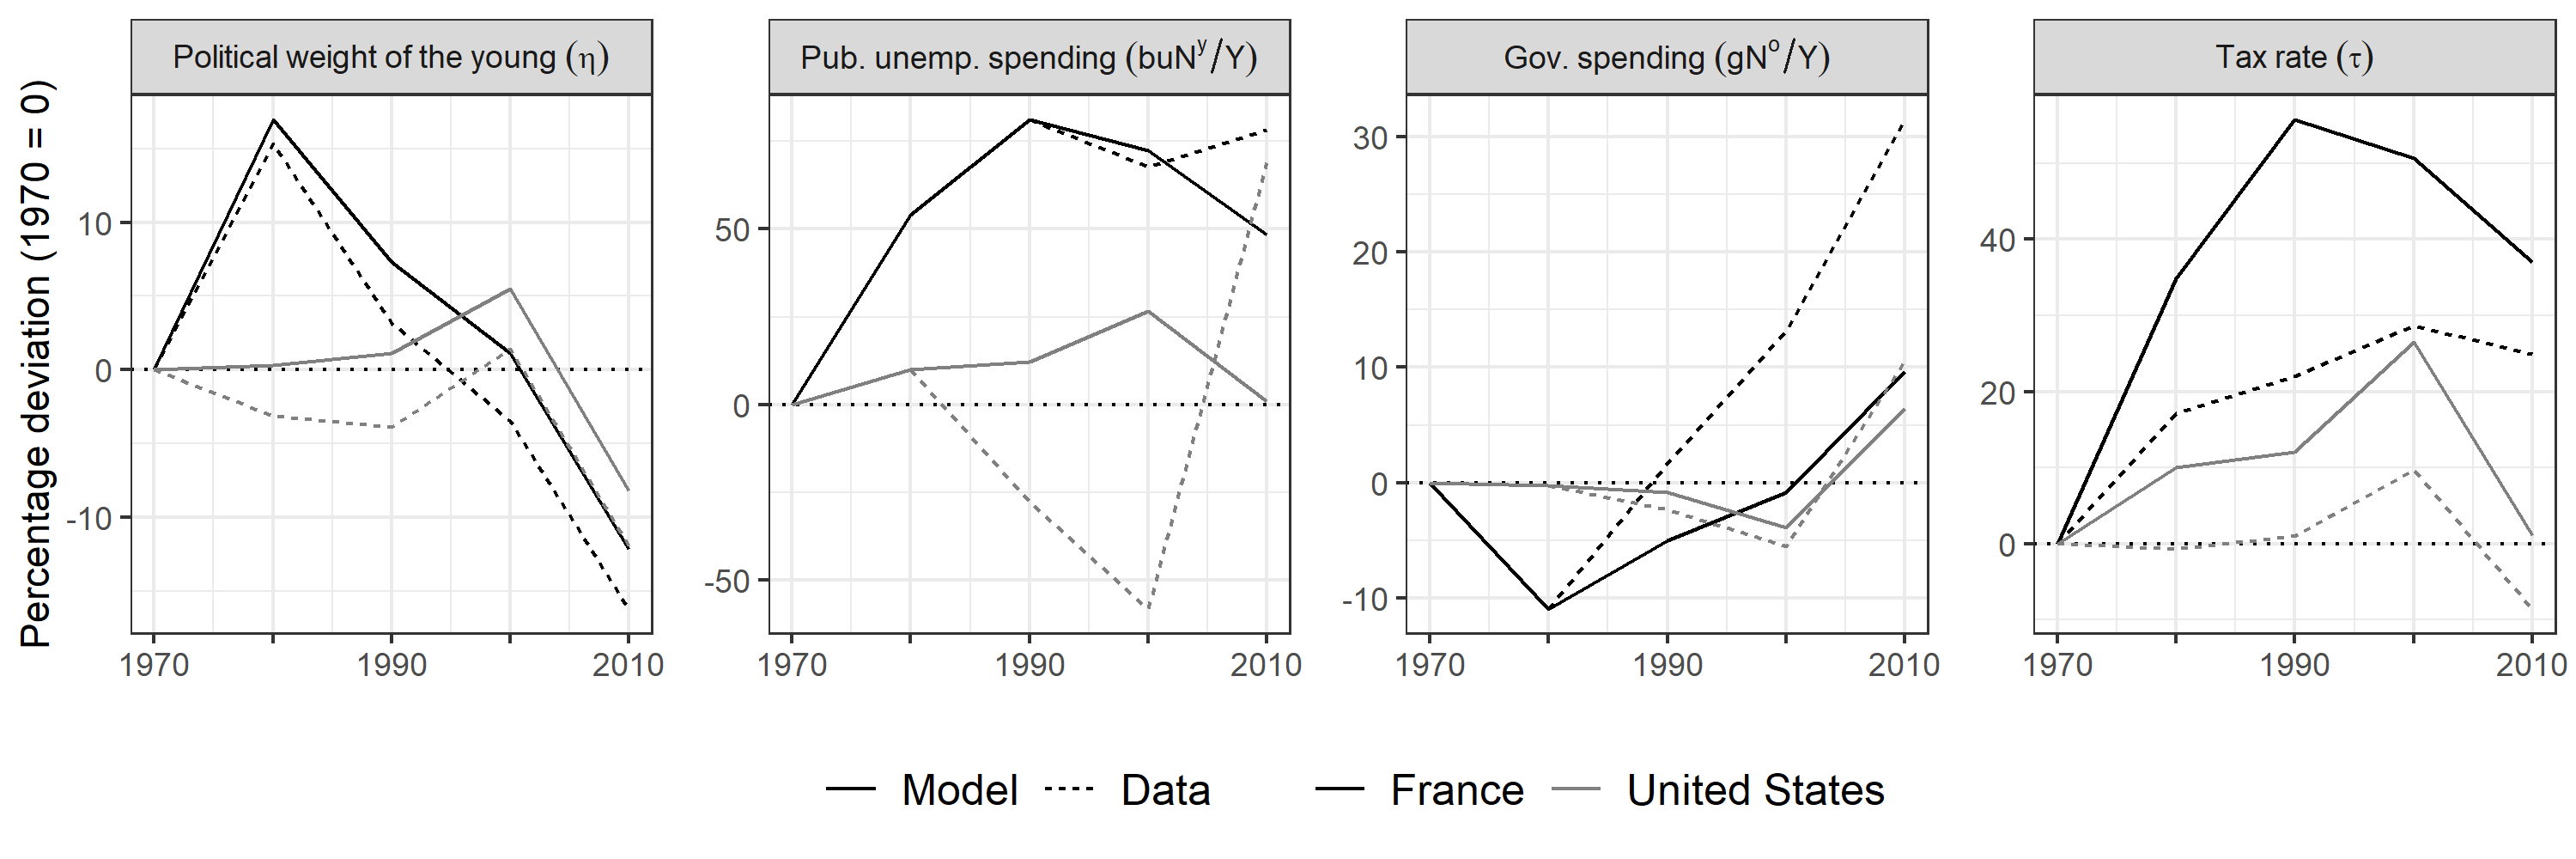
\includegraphics[width=1\linewidth]{chap1/graphic/quant-bench-dev7010-pub.png}
	\vspace{-3em}
	\justify\singlespacing\footnotesize\textit{Notes:} The figure shows the deviation of the variables from the public policy equilibrium from their 1970's value (in percentage) for France and the United States over the 1970-2010 period. Solid lines represent the dynamics obtained from the model simulation, dashed  lines represent the data, and the dotted line represents the 0-degree line.
\end{figure}
% Demographic context (n and p)
The rate of population growth $n_t$ slightly exceeds the increasing survival rate $p_t$ between 1970 and 2000. Thus, the old-age-dependency ratio $p_t/n_t$ remains roughly stable, although it declines slightly in France between 1980 and 1990 due to the massive entry of the boomers into the labor force. The old-age-dependency ratio starts to increase around 2000 due to a steady population growth combined with a sharply increasing survival rate, the boomers' generation starting to retire. As a result of this demographic context, the political weight of the young $\eta_t$ is above its 1970's level until 2000 in both countries as depicted in the first panel of the figure.

As the political weight of the young boomers rises, pro-youth policies are implemented due to the opportunistic behavior of political parties. These policies consist of more redistribution, i.e. a greater tax rate and more unemployment benefits, to prevent the income losses due to unemployment of the young boomers. Thus, the old-age specific government spending also decline, before increasing again as the boomer cohort starts to retire in 2010. Since the unemployment benefits act as an outside option for the workers, these public policy dynamics have consequences on the labor market.

Figure \ref{chap1-fig:quant-bench-dev7010-labor} displays the dynamics of labor market variables, expressed in percentage deviation from their 1970's value.
\begin{figure}[!tb]
	\centering
	\caption{Labor market dynamics over the 1970-2010 period} \label{chap1-fig:quant-bench-dev7010-labor}
	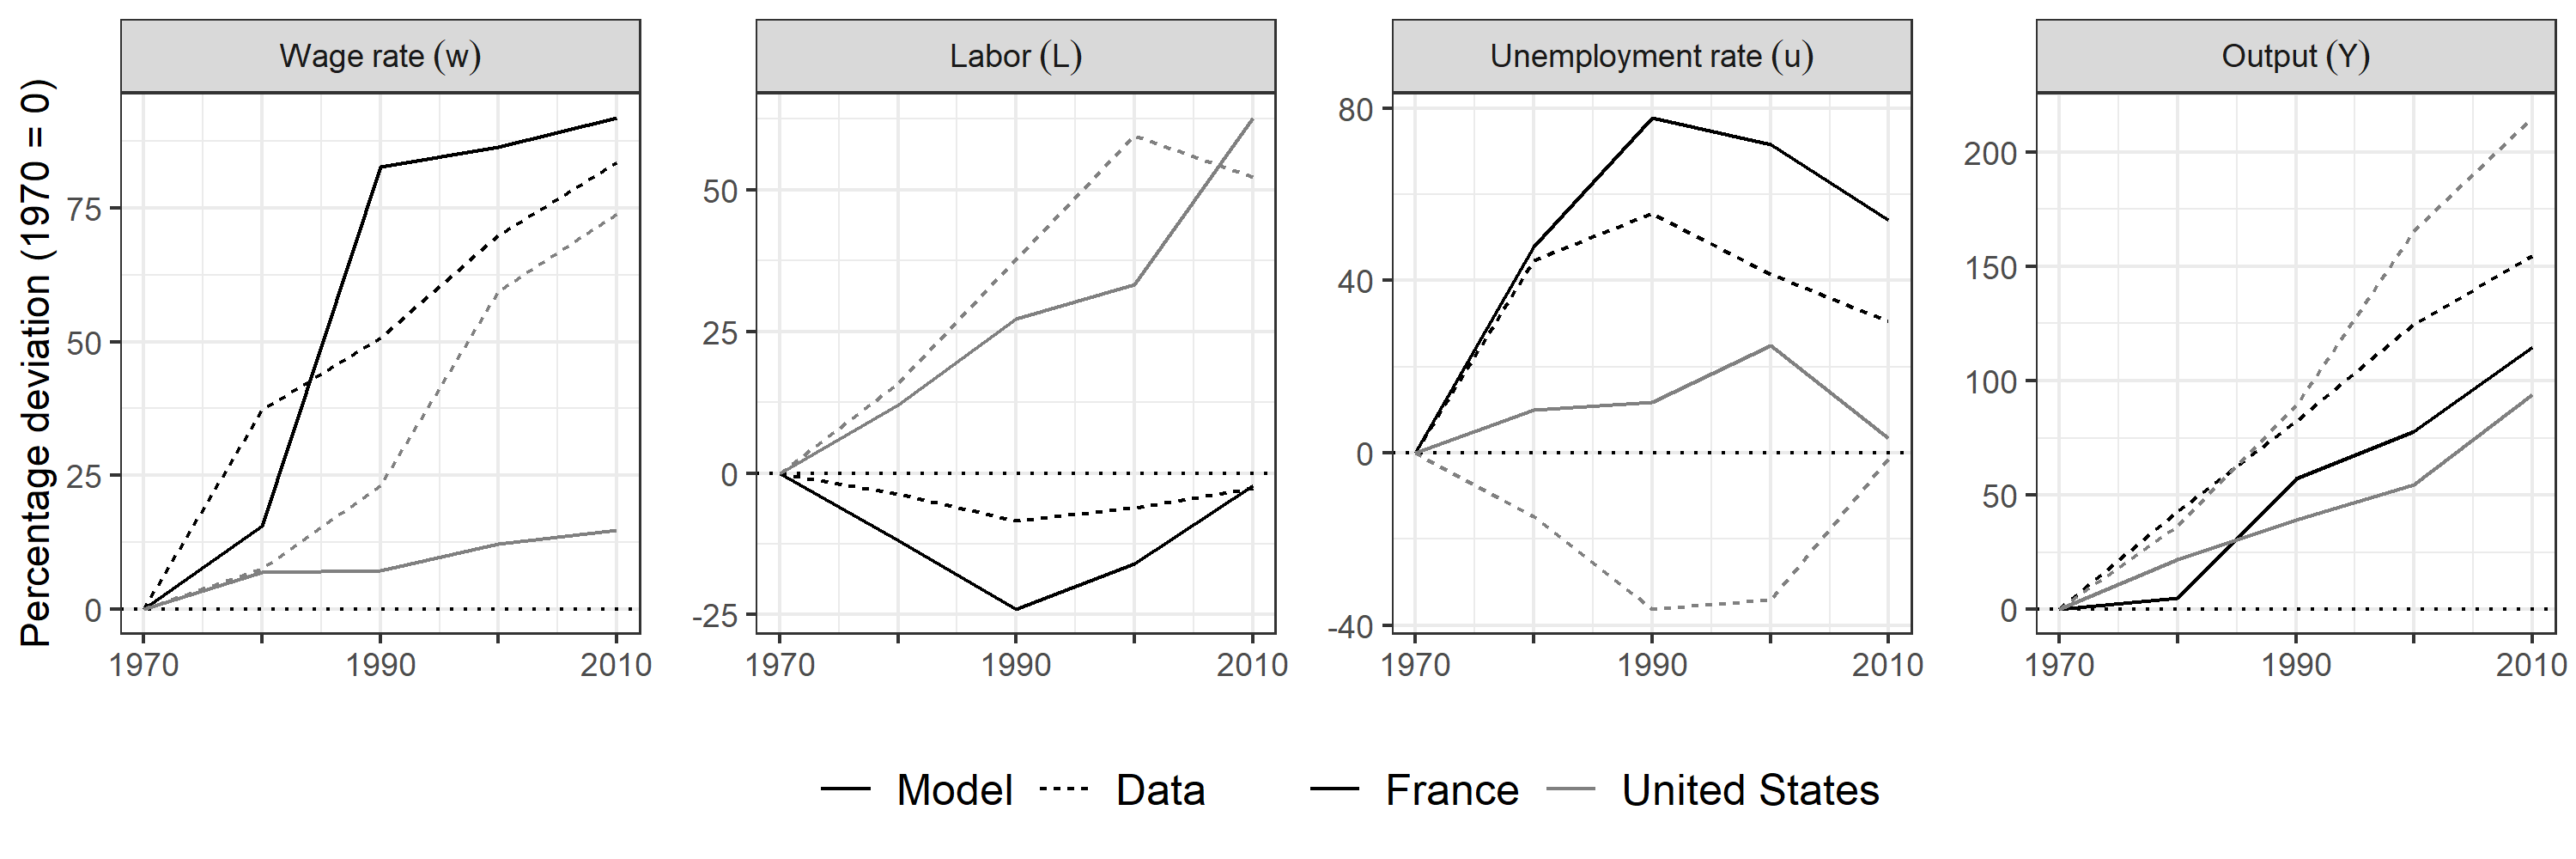
\includegraphics[width=1\linewidth]{chap1/graphic/quant-bench-dev7010-labor.png}
	\vspace{-3em}
	\justify\singlespacing\footnotesize\textit{Notes:} The figure shows the deviation of the variables from the labor market equilibrium from their 1970's value (in percentage) for France and the United States over the 1970-2010 period. Solid lines represent the dynamics obtained from the model simulation, dashed  lines represent the data, and the dotted line represents the 0-degree line.
\end{figure}
Workers can bargain greater wages as their outside option increases. Because the labor cost (i.e. the wage) increases for firms, they shift away from labor. This behavior is permitted by two features of the model. 
First, the monopsony position of the firm in the labor market enables the firm to hire and fire as much as wanted. 
Second, the capital-labor elasticity of substitution $\sigma$ is greater than one, thus, both input factors are gross substitutes and the firm is all the more able to substitute labor with capital for a given output level. This behavior leads to a decline of the number of workers $L_t$ in France and a moderate increase in the US, as highlighted in the second panel. The diverging patterns between the two countries are due to the substitution effect being stronger in France than in the US. The higher elasticity of substitution in France combined with faster growth of the capital stock $K_t$ pushes French firms to substitute relatively more labor with capital. Thus, the number of workers becomes lower than its 1970's level in France, whereas the US manage to slightly increase their labor factor because the increase in wages is not as strong as in France.

This fall in employment raises unemployment in France, the effect being enhanced by the labor force growth due to the number of young boomers. For the US, the moderate increase in labor does not manage to offset population growth. Therefore, the unemployment rate also raises as depicted in the third panel. Since both factors are gross substitutes, output $Y_t$ and output-per-worker grow along with capital-per-worker. The increase in output per worker exceeds the one of the wages, and as a result, the labor share declines.

The mechanisms until 2010 can be summarized as follows. The young boomers change labor market institutions in their favor due to their relatively high political weight. This raises the outside option of workers and hence their bargaining power, enabling them to bargain greater wages. Labor becoming costly, firms decide to shift away toward capital. This shift-away from labor engenders an increase in output-per-worker that exceeds the wage gain; thus, the labor share declines. 

\textbf{The retired boomers (2010-2050) and afterward (2050-2100).} Dynamics of the same set of variables also help to highlight the mechanisms of the model's predictions for the labor share after 2010.
Figure \ref{chap1-fig:quant-bench-dev1000-pub} displays the dynamics of public policy variables, expressed in percentage deviation from their 2010's value.
\begin{figure}[!tb]
	\centering
	\caption{Public policy dynamics over the 2010-2100 period} \label{chap1-fig:quant-bench-dev1000-pub}
	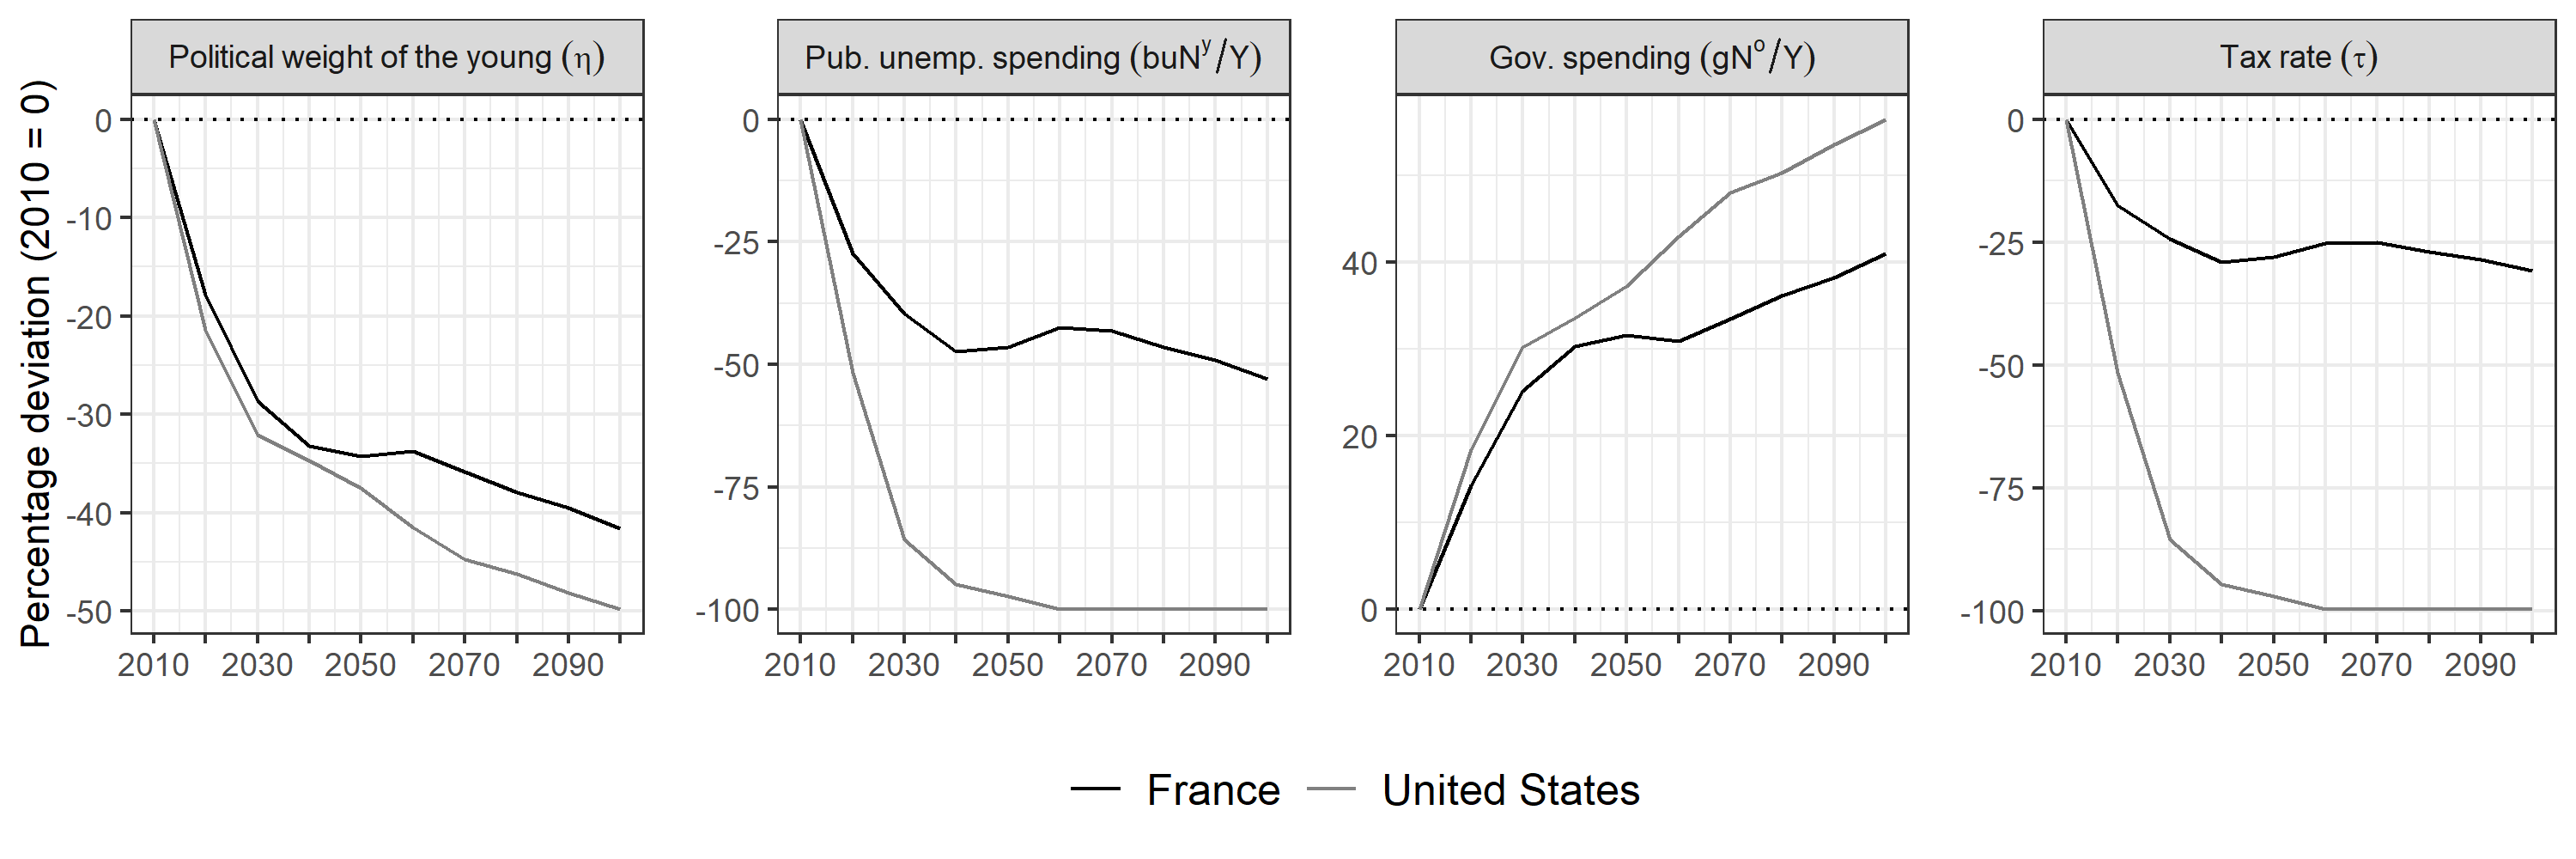
\includegraphics[width=1\linewidth]{chap1/graphic/quant-bench-dev1000-pub.png}
	\vspace{-3em}
	\justify\singlespacing\footnotesize\textit{Notes:} The figure shows the deviation of the variables from the public policy equilibrium from their 2010's value (in percentage) for France and the United States over the 2010-2100 period. Solid lines represent the dynamics obtained from the model simulation and the dotted line represents the 0-degree line.
\end{figure}
The demographic context over this period is the following: the rate of population growth $n_t$ declines sharply between 2010 and 2050 before stabilizing thereafter. Meanwhile, the survival rate $p_t$ grows by around 4\% per decade. Thus, the old-age-dependency ratio sharply increases from 2010 to 2050. Once the rate of population growth becomes stable, the old-age-dependency ratio still grows but at a lower rate. As a result, the political weight of the young, $\eta_t$, never returns to its 2010 level and strongly declines until 2050 for both countries as shown in the first panel.

As the political weight of the young declines, the reverse of the mechanism that led to the decline of the labor share when the boomers were young is expected. Opportunistic political parties favor the retired boomers and implement pro-elderly public policies, i.e. a lower tax rate and more old-age specific government spending. Thus, unemployment benefits decline and so does the outside option of workers. These changes in public policy have consequences on the labor market.

Figure \ref{chap1-fig:quant-bench-dev1000-labor} displays the dynamics of public policy variables, expressed in percentage deviation from their 2010's value.
\begin{figure}[!tb]
	\centering
	\caption{Labor market dynamics over the 2010-2100 period} \label{chap1-fig:quant-bench-dev1000-labor}
	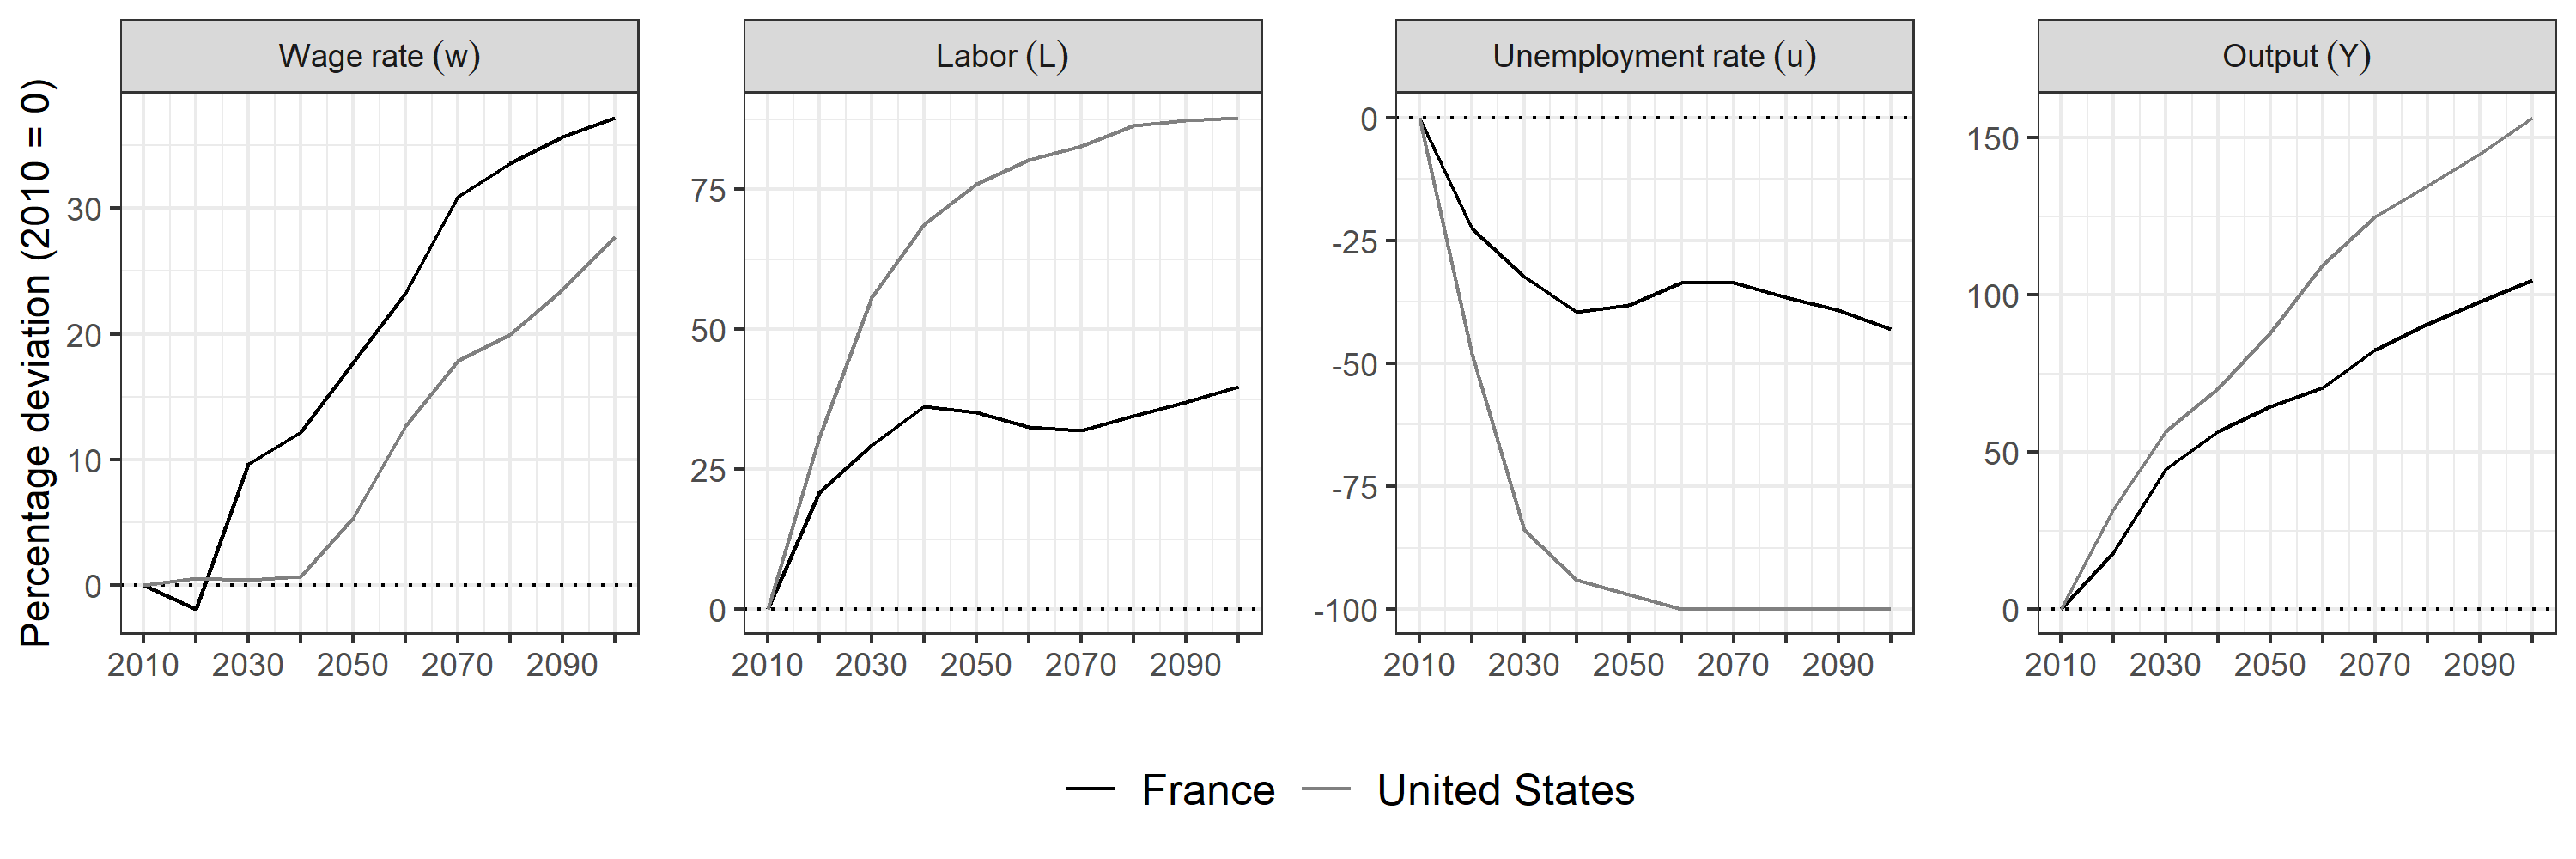
\includegraphics[width=1\linewidth]{chap1/graphic/quant-bench-dev1000-labor.png}
	\vspace{-3em}
	\justify\singlespacing\footnotesize\textit{Notes:} The figure shows the deviation of the variables from the labor market equilibrium from their 2010's value (in percentage) for France and the United States over the 2010-2100 period. Solid lines represent the dynamics obtained from the model simulation and the dotted line represents the 0-degree line.
\end{figure}
As a result, they concede a wage stagnation inciting firms to hire more, as depicted in the second panel. The unemployment rate drops due to higher employment combined with the decline of the rate of population growth, as shown in the third panel.

Nonetheless, the labor share never recovers its 2010's level. The dynamics of the labor share are governed by two factors: an increase in employment and a higher capital stock arising from the savings of the boomers when they were young. These savings were fostered by the size of the boomer generation; the rising expected life expectancy; and the high level of their wages. While higher employment tends to increase the labor share, the larger stock of capital tends to reduce it, keeping the labor share roughly stable in both countries when the boomers are retired.

Once the boomers pass away, after 2050, the decline in the political power of the young slows down in both countries. This slowdown allows workers to bargain greater wages. French firms substitute labor with capital to thwart workers' appropriation of the rents, leading to a decline of the labor factor and so a rise in unemployment. On the other side of the Atlantic, firms in the US manage to hire until full-employment due to the sharp increase in capital and the stagnation of the labor supply. However, the wage gains remain lower than the rise in output-per-worker in both countries. Therefore, both labor shares decline to reach 60.4\% in France and 58.8\% in the US by 2100, while their respective levels were about 64.5\% and 62.8\% in 2010.

The mechanisms after 2010 can be summarized as follows. The boomers retire and change the public policy in their favor, reducing taxes and unemployment benefits which raises employment. The positive effect of employment on the labor share is dampened by capital accumulation due to the extensive savings of the boomers when they were young. Consequently, the labor share slightly increases in France and stabilizes in the US, before declining again by the end of the century due to the aging of the population.

\subsection{Factor-accumulation and policy-mechanism effects} \label{chap1-counterfactual}

% Mechanisms so far
So far I have highlighted the different mechanisms through which the age structure of the population affects economic variables and therefore the labor share. Demographic changes are due to changes in two exogenous variables: the population growth rate $n_t$ and the survival rate $p_t$. 
Their dynamics may affect the labor share through two channels: the \textit{direct factor-accumulation} effect and the \textit{indirect policy-mechanism} effect.

% Quantify
To quantify the respective role of each effect, I make counterfactual simulations. In these simulations, I neutralize a channel of demographic changes by setting it to its level in 1970, i.e. the decade before the massive entry of the boomers on the labor market.
% Initial values
Table \ref{chap1-tab:quant-demo70} summarizes the demographic variables in 1970.
\begin{table}[!tb]
    \centering
    \begin{threeparttable}
        \caption{Demographic variables in 1970} \label{chap1-tab:quant-demo70}
        
\begin{tabular}{llrr}
\toprule
\textbf{} & \textbf{Variable} & \textbf{France} & \textbf{United States}\\
\midrule
$n_{1970}$ & Population growth rate & 1.134 & 1.597\\
$p_{1970}$ & Survival rate & 0.417 & 0.476\\
$p_{1990}$ & Expected survival rate & 0.583 & 0.561\\
$\frac{p_{1970}}{n_{1970}}$ & Old-age dependency ratio & 0.368 & 0.298\\
$\eta_{1970}$ & Young political weight of the young & 4.169 & 2.869\\
\bottomrule
\end{tabular}

        \begin{tablenotes}[flushleft]
            \footnotesize{\item \textit{Notes}: The table reports the demographic variables in 1970 for France and the United States. 
            % Data are from the benchmark simulation of the model.
            }
        \end{tablenotes}
    \end{threeparttable}
\end{table}
Then, I compare counterfactual simulations to the benchmark obtained in section \ref{chap1-model_pred}, thus, I quantify to which extent each channels affect the labor share. For more details on the methodology to construct the counterfactual simulations, see appendix \ref{chap1-countermetho}.

% Direct vs indirect
To neutralize the factor accumulation effect, I suppose that all demographic parameters remain at their 1970's level, i.e. $n^\prime_t = n_{1970}$ and $p^\prime_t = p^\prime_{t+1} = p_{1970}$, which affects population dynamics and the saving rate. In this simulation, only the political weight of the young remains identical to the benchmark simulation, i.e. $\eta_t^\prime = \eta_t$. Conversely, I neutralize the policy mechanism effect by setting the political weight of the young to its level in 1970, i.e. $\eta^\prime_t = \eta_{1970}$, while all demographic parameters remain at their benchmark values. Lastly, I make a counterfactual simulation to neutralize both channels in which $n^\prime_t = n_{1970}$, $p^\prime_t = p^\prime_{t+1} = p_{1970}$ and $\eta_t^\prime = \eta_{1970}$. This latter simulation is the baseline counterfactual simulation.

% Figure for direct vs indirect
Figure \ref{chap1-fig:quant-decomp-channel} presents the sizes of the factor accumulation effect and the policy mechanism effect, derived from the counterfactual simulations, in percentage points.
\begin{figure}[!tb]
	\centering
	\caption{Decomposition of the channels of demographic changes} \label{chap1-fig:quant-decomp-channel}
	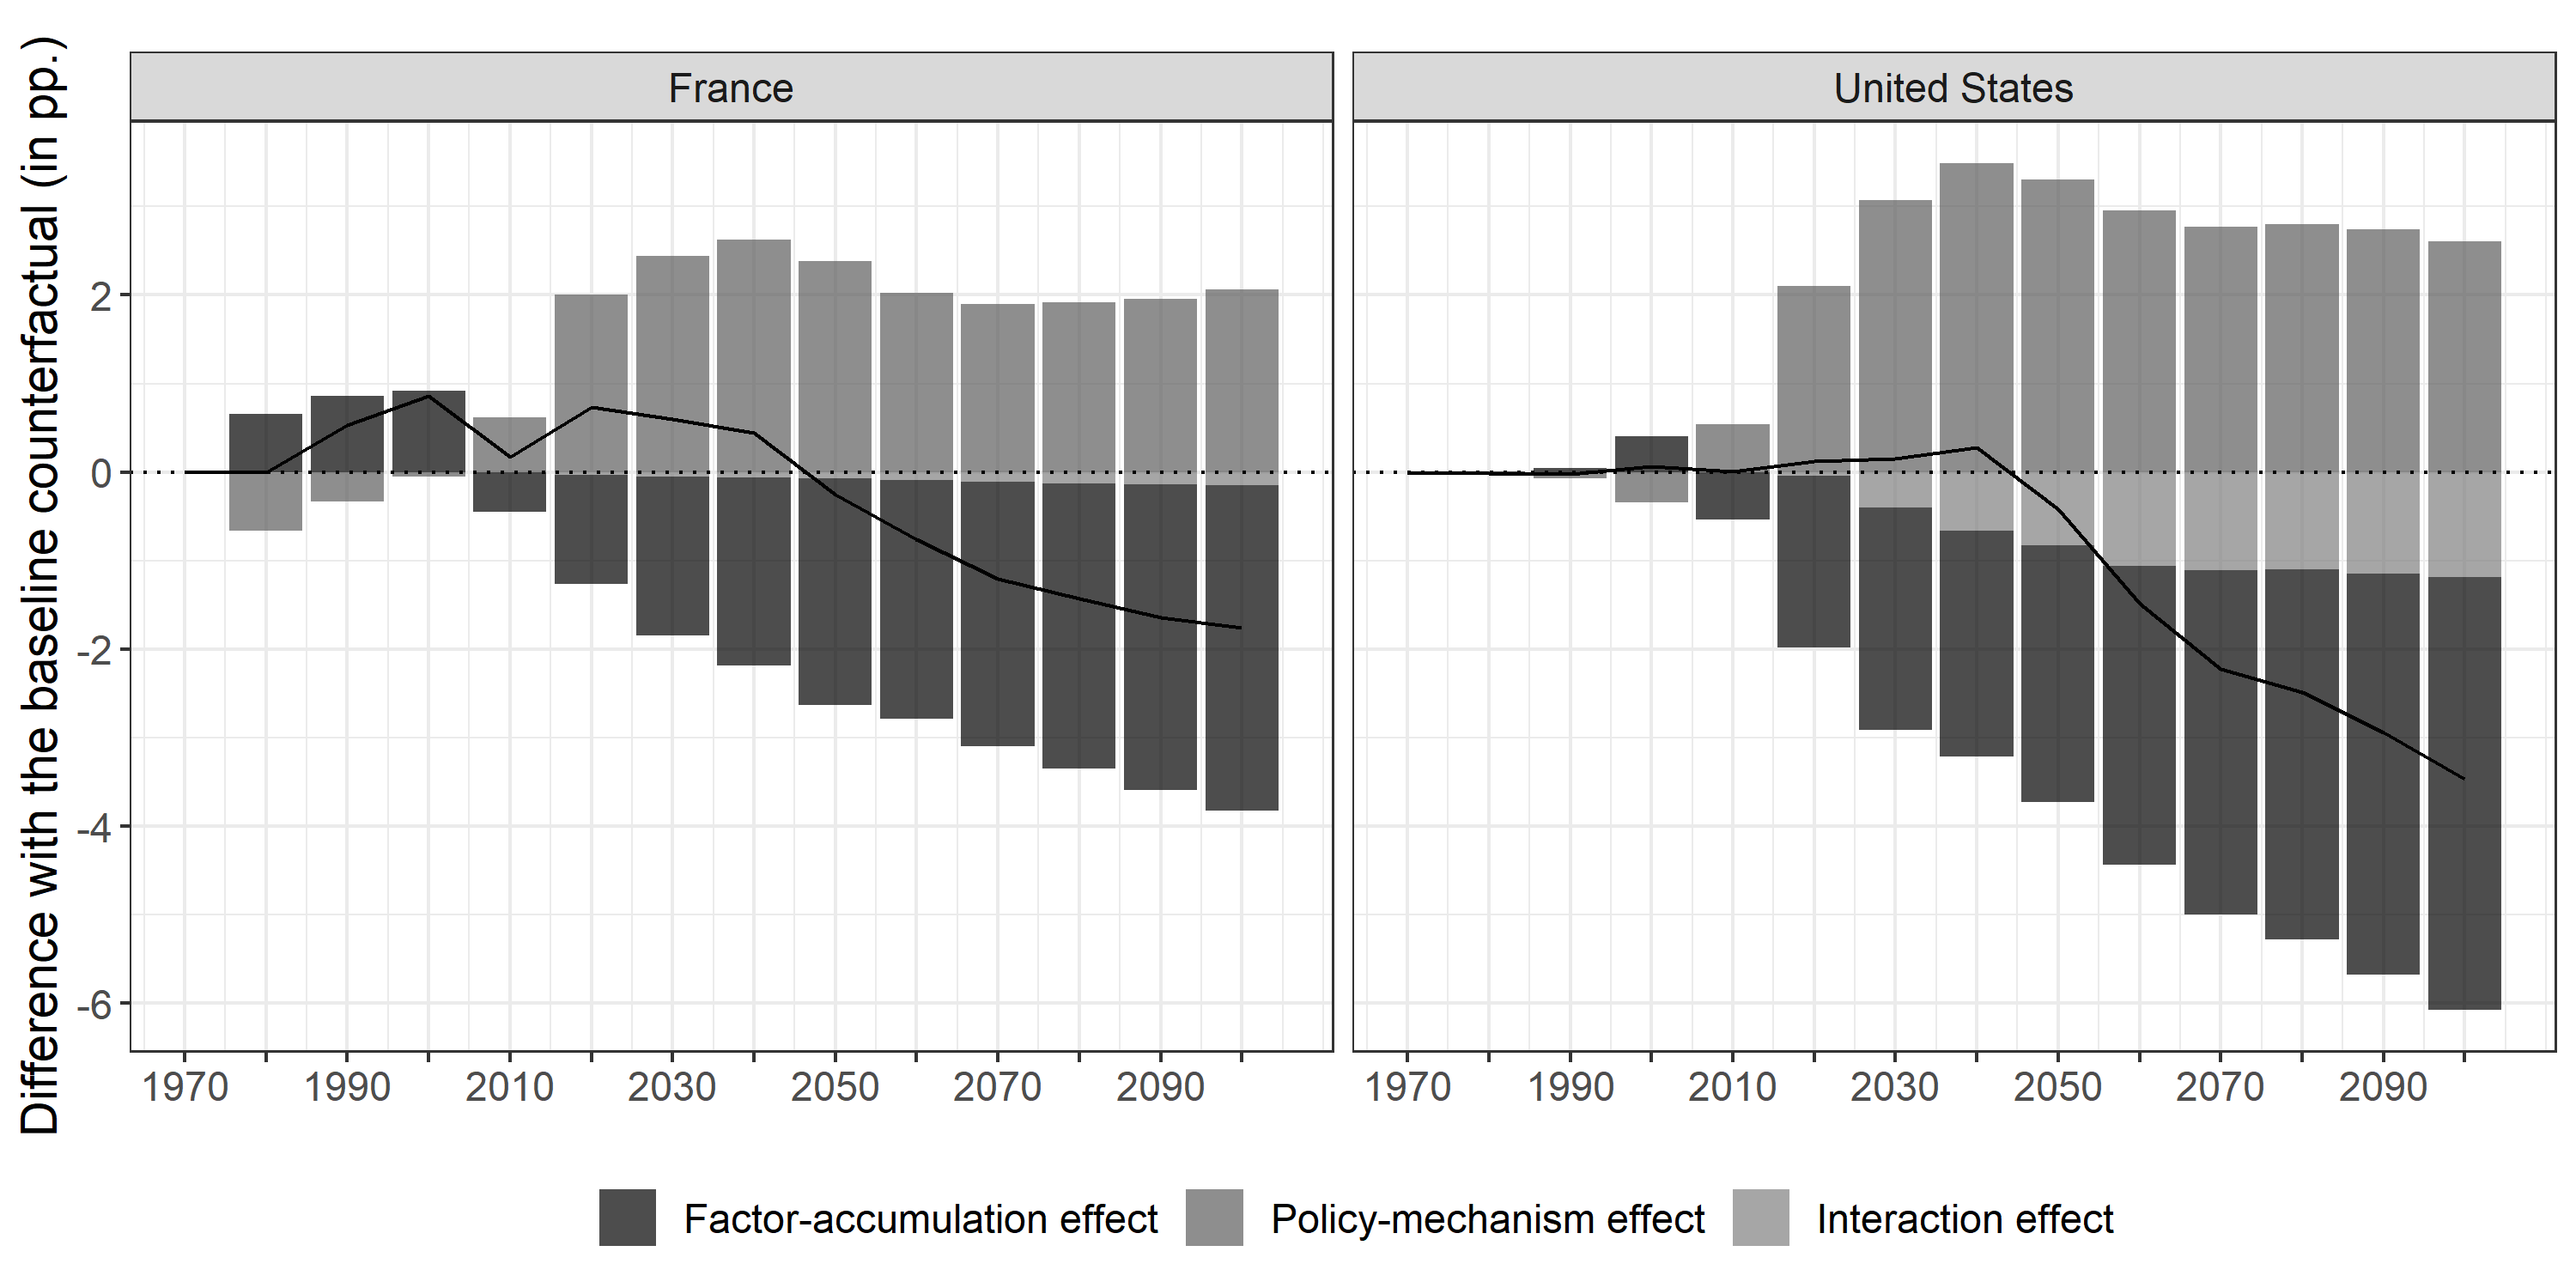
\includegraphics[width=1\linewidth]{chap1/graphic/quant-decomp-channel.png}
	\vspace{-3em}
	\justify\singlespacing\footnotesize\textit{Notes:} The figure shows the decomposition of the channels of demographic changes on the labor share. Effects are expressed in percentage point difference with the baseline counterfactual simulation. The baseline counterfactual corresponds to the simulation where all the demographic variables and the young political weight remain at their initial levels. The factor-accumulation effect accounts for the effect of demographic changes through the factor-accumulation channel on the labor share, while the policy-mechanism effect accounts for the effect of demographic changes through the policy-mechanism channel. Both effects are obtained by taking the difference between the benchmark labor share and the labor share from the simulation in which the channel is canceled. The interaction effect is defined as the part which is not exclusively explained by both effects independently. The solid line represents the net effect corresponding to the sum of the three effects, that is also the difference between the labor shares from the benchmark and the baseline counterfactual simulation.
\end{figure}
% Direct mostly positive % Increasing Ny => low wages => increases L
The factor-accumulation effect is mostly positive when the boomers are young, because the increasing labor supply is in favor of firms within the bargaining, keeping wages low which fosters employment. 
% In addition, the saving rate remains low and so does the capital stock.
Meanwhile, the policy-mechanism effect harms the labor share, owing to the rise of the young boomers' political weight which increases their unemployment benefits, hence wages, and therefore incites firms to shift away from labor toward capital.

% AFTER 2010: boomers retire, both effects are reversed
Once the boomers start to retire in 2010, both effects are reversed. The policy-mechanism effect becomes positive because old boomers foster pro-elderly public policy. This change in the policy is done at the cost of labor market insurance. Thus, workers are not able to bargain greater wages which fosters labor demand. Nonetheless, the factor-accumulation effect is negative because of the large amount of available capital stock due to the savings of the boomers when they were young. As a result, the factor-accumulation effect offsets the positive impact on the labor share of the reversal policy-mechanism effect.

% % \textbf{Summary of the effects.} 
% Figure \ref{chap1-fig:quant-decomp-sum} summarizes the relative share of the effects of demographic changes on the labor share by period and country.
% \begin{figure}[!tb]
% 	\centering
% 	\caption{Relative share of the effects of demographic changes on the labor share} \label{chap1-fig:quant-decomp-sum}
% 	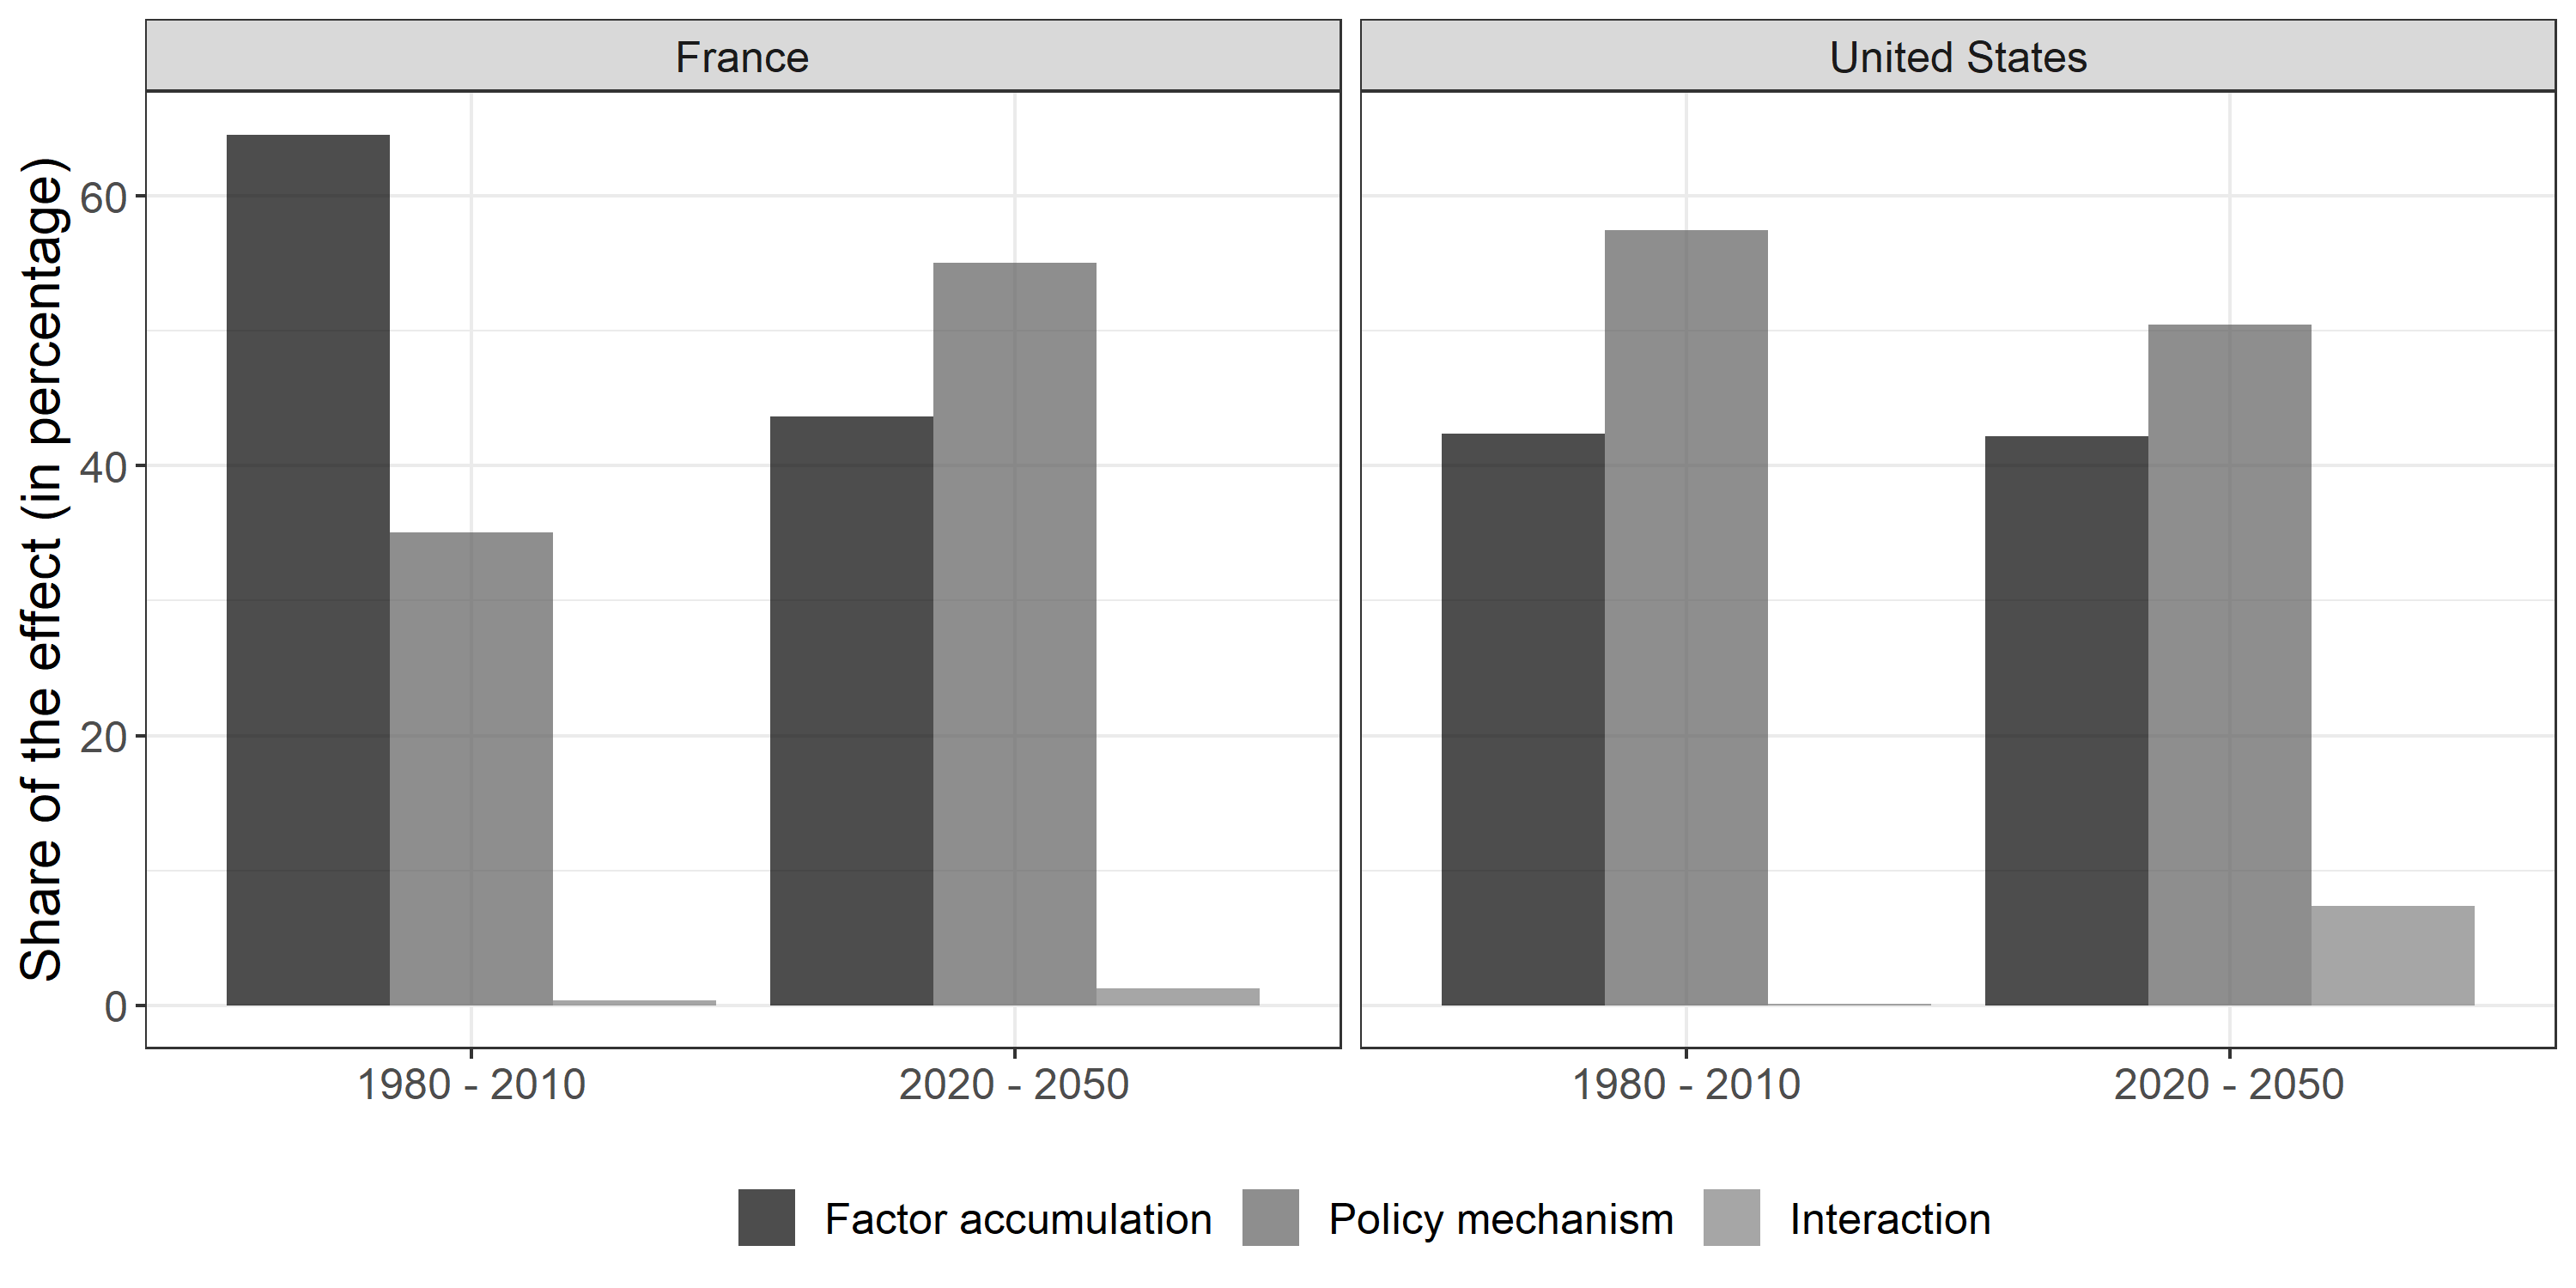
\includegraphics[width=1\linewidth]{chap1/graphic/quant-decomp-sum.png}
% 	\vspace{-3em}
% 	\justify\singlespacing\footnotesize\textit{Notes:} The figure shows the average percentage relative share of the channels of demographic changes on the labor share over the two periods of the boomers generation (young and old), for France and the United States. Data are from the counterfactual simulations of the model and summarize the results from figure \ref{chap1-fig:quant-decomp-channel}.
% \end{figure}
% Changes in the population growth rate and survival rate affect the labor share through two channels: the factor-accumulation effect and the policy-mechanism effect. When the boomers are young, the factor-accumulation effect dominates in France while the policy-mechanism effect prevails in the US. On average, the share explained by the policy-mechanism effect is about 35\% in France and 57.5\% in the US. Thereafter, between 2020 and 2050, the share of this latter effect rises by 20.8 pp. in France becoming the main channel, while it slightly decreases by 7 pp. in the US. These results suggest that the policy-mechanism effect accounts for more than half of the consequences of demographic dynamics on the labor share.

% Compare with SV2013
\citet{Schmidt2013Demographic} consider only the factor accumulation mechanism and show that this mechanism disappears in a small open economy because capital-per-worker and the wage rate are independent of domestic savings, so that labor share dynamics only reflect changes in net foreign assets.
% My approach
The major advantage of my approach is that the policy mechanism holds in a small open economy.
%
With capital mobility, \citet{Pica2010Capital} argues that competition to attract capital between countries leads to reduced labor market regulation and a lower labor share.
%
Nonetheless, he uses a Cobb-Douglas production function which cancels out the shift away from labor toward capital of firms that is allowed by the CES production function that I employ.
%
In terms of consequences for the labor share, the effect of capital markets integration that occurs through labor market deregulation in an open economy is equivalent to the response of the firms that substitute labor with capital to thwart workers' appropriation of the rents in a closed economy.

\subsection{Age-related conflict: who are the winners ?} \label{chap1-winners}

% So far
The results show that the labor share declines due to the size of the boomers' cohort in France and the US. First, when they are young they shape labor market institutions in their favor, raising wages but inciting firms to shift away from labor toward capital. Second, when they are old they have substantially increased the available capital in the economy through their savings, pushing firms to substitute even more. Although it may seem obvious that the boomers are the winners of the age-related conflict when they are old, the results raise the question of whether they were the losers when they were young because the labor share declined considerably over this period.

Although much emphasis is given to it in the policy debate, the labor share is a gross indicator of the income distribution that does not take into account redistribution. The net income ratio between young and old is more appropriate to determine the winners of the age-related conflict.\footnote{I do not consider the difference in lifetime utility between generations to assess who are the winners. The shape of the utility function does depend on the date at which a generation appears because the effective discount factor $\alpha p_{t+1}$ depends on life expectancy which varies across generations. Since two generations do not have the same baseline, then utility comparisons do not make much sense.}
Let $T$ be the per-capita redistribution from old to young that is the product between the old-age dependency ratio, i.e. $p_t/n_t$, and the difference between the after-tax and before-tax young-to-old income ratios, i.e. $Y_t^y/Y_t^o - \Theta_t$. Using equation \eqref{chap1-eq:after-tax-income-ratio},
\begin{equation*}
    T_t \equiv \frac{p_t}{n_t}\left(\frac{Y_t^y}{Y_t^o} - \Theta_t\right) =  \frac{p_t}{n_t}\left(\eta_t - \Theta_t\right).
\end{equation*}
Therefore, changes in per-capita redistribution reflect changes in the old-age dependency ratio, i.e. $p_t/n_t$, and in the aggregate redistribution, i.e. $\eta_t - \Theta_t$.

Figure \ref{chap1-fig:discuss-ratiopc} presents the per-capita redistribution from old to young in percentage deviation from its value in 1970.
\begin{figure}[!tb]
	\centering
	\caption{Per-capita redistribution dynamics} \label{chap1-fig:discuss-ratiopc}
	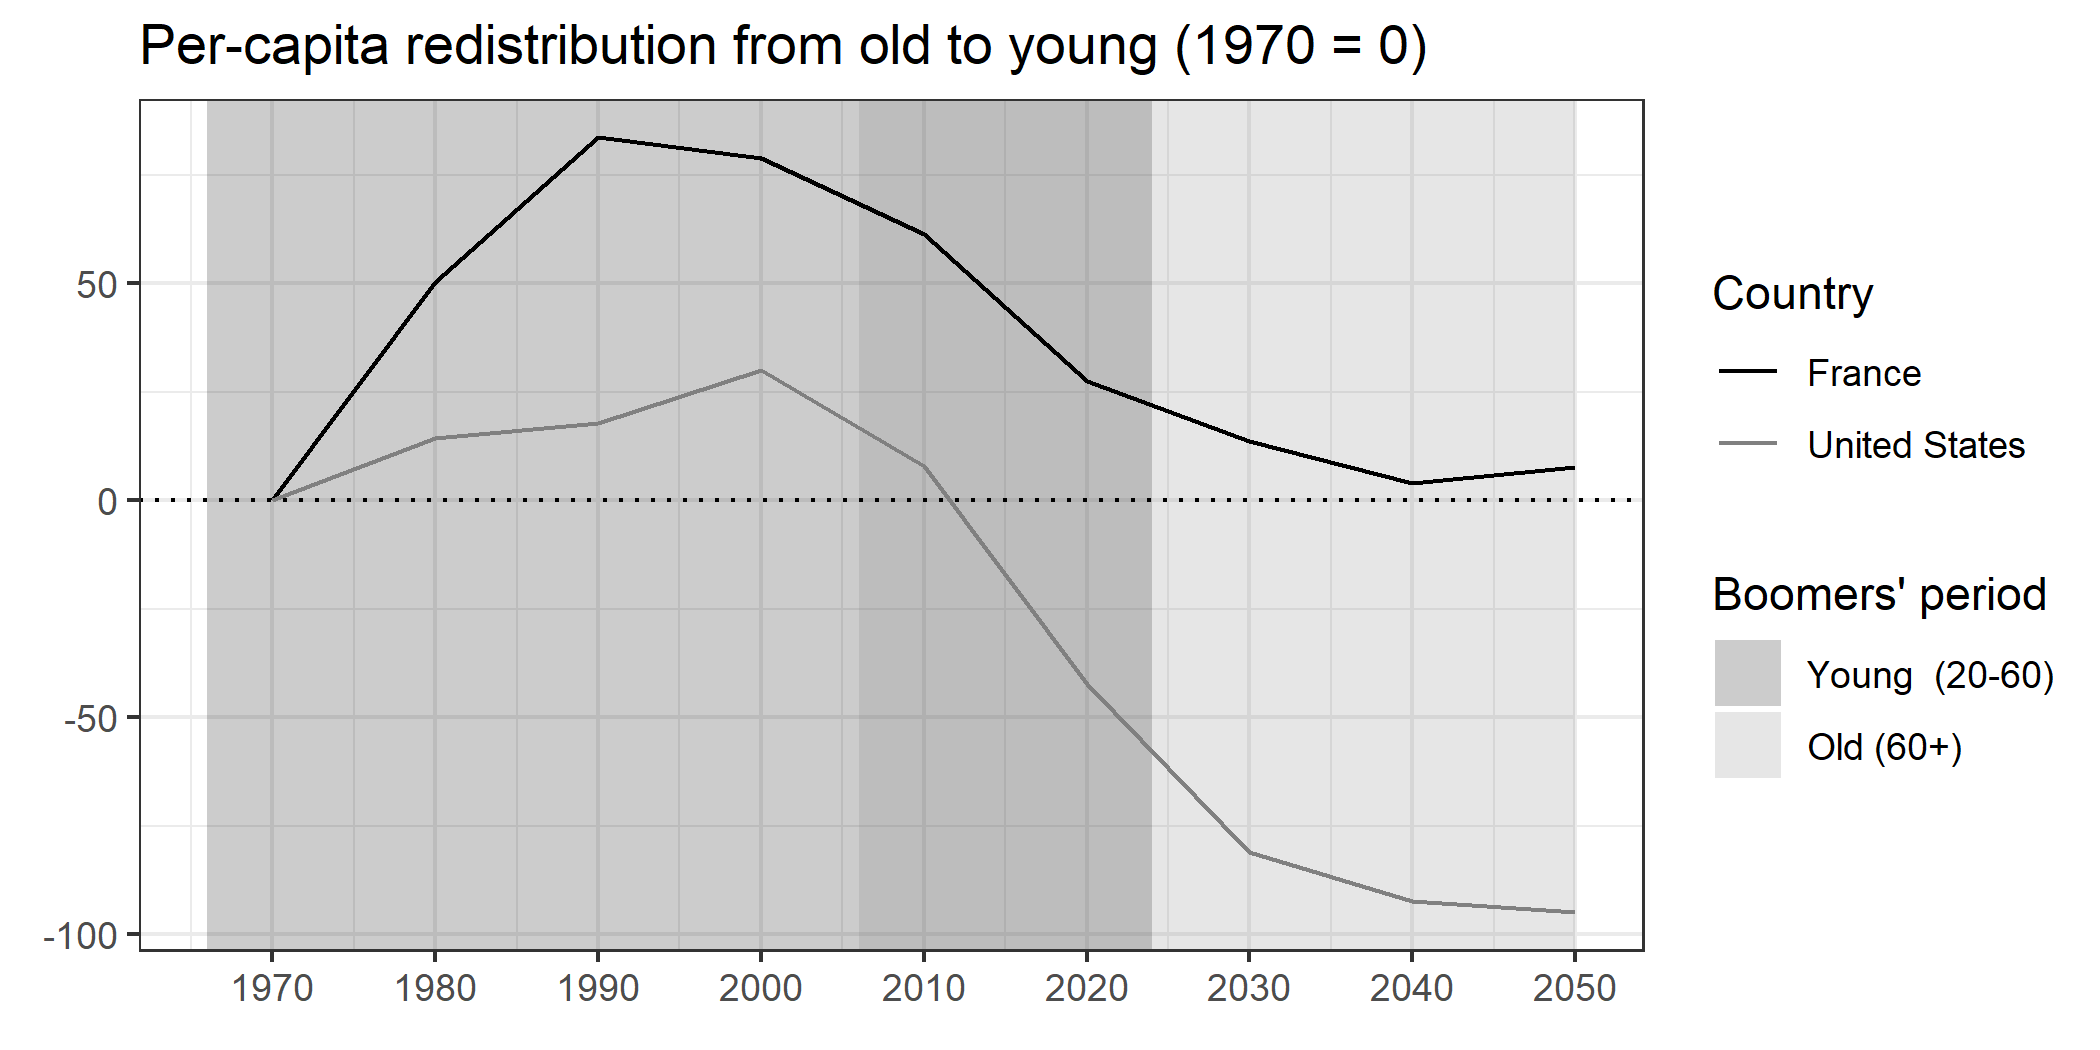
\includegraphics[width=1\linewidth]{chap1/graphic/discuss-ratiopc.png}
	\vspace{-3em}
	\justify\singlespacing\footnotesize\textit{Notes:} The figure shows the per-capita redistribution from old to young for France and the United States in percentage deviation since 1970. The black and grey lines represent, respectively, the France and the United States. The dotted line represents the 0-degree line. Rectangles define the periods when the boomers are young and old. Data are from the benchmark simulation of the model.
\end{figure}
When the boomers are young and enter the labor market (in 1970), they earn labor income until they start to retire in 2010. Over this period, the labor share declines and the per-capita redistribution from old to young increases in both countries. The young boomers are the winners of the age-related conflict over this period because they manage to recover their labor income losses by increasing redistribution due to their political weight. Once they retire and earn capital income, the labor share is rather stable, although the per-capita redistribution sharply declines. As a result, the boomers are also the winners of the age-related conflict when they are old because the level of redistribution from old to young declines. In the case of the US, the redistribution from old to young tends toward zero as the US economy is in full employment, hence, there is little need for unemployment benefits.\footnote{Note that the only source of heterogeneity is age, thus, there may be winners and losers within each cohort in presence of additional dimensions of heterogeneity, e.g. human capital.}
    
    \section{Conclusion} \label{chap1-conclusion}
    %% SUMMARY OF PAPER IDEAS AND MODEL
A vast literature emphasizes the role of biased technical change and institutions to explain the shift from labor toward capital and therefore the decline of the labor share observed in several countries over the past few decades. This paper focuses upstream of these determinants and highlights the role of demography as a force that shapes labor market institutions and hence the allocation of factor incomes. These institutions define the rules of the game for wage bargaining between firms and workers. When a particular generation, such as the boomers, can change institutions in its favor, then these rules also change, which affects the allocation of income between capital and labor. This mechanism accounts for the indirect \textit{policy-mechanism} effect of demographic changes on the labor share that results from the inter-generational conflict when choosing the public policy. Besides, the age structure of the population also has a direct \textit{factor-accumulation} effect that occurs through the labor supply and capital stock. Both effects combined help understand the role of the boomers' cohort in the decline of the labor share in France and the United States.

This paper shows to which extent we should take into account changes in institutions, that are endogenously determined by the age structure of the population, to understand macroeconomic dynamics in the long run. Decomposing the direct factor-accumulation effect and the indirect policy-mechanism effect, I find that the latter is as important as the former in explaining how demographic dynamics affect the labor share. Thus, omitting this indirect mechanism, and more broadly supposing that institutions do not change in the long run, leads to underestimating the role of demography on the factor income distribution. In this regard, my results provide a new conceptual framework to examine demographic dynamics and institutions in future work.

%% IMPLICATIONS IN TERMS OF POLICY DEBATE
These results have implications in terms of current policy debates. On the one hand, several high-income countries have experienced aging of their population which has led to a debate about optimal public policy. In this respect, my results shed light on the consequences of demographic changes on the allocation of income between capital and labor. On the other hand, developing countries are witnessing large demographic changes and may experience the arrival of a generation such as the boomers' cohort, which would change their institutions along with factor shares, and therefore, may have consequences on their development.
    
    %%% DO NOT CHANGE %%%
    \printbibliography[heading=subbibintoc]
    
    \clearpage
    \addsec{Appendices}
    \renewcommand{\thesubsection}{\thechapter.\Alph{subsection}}
    %%% DO NOT CHANGE %%%
    
    %%% APPENDICES
    
    \subsection{Probabilistic voting} \label{chap1-probabilistic}
    In order to determine their preferred public policy, households maximize their indirect utility function. Using the first order conditions from the household maximization problem in equations \eqref{chap1-eq:hhmaxc1}, \eqref{chap1-eq:hhmaxc2} and \eqref{chap1-eq:hhmaxs}, I obtain:
\begin{align}
	U_t^{y,i} &= \ln\left[\frac{1}{1+\alpha p_{t+1}}y_t^i\right]+ \alpha p_{t+1} U_{t+1}^{o,i}, \label{chap1-eq:utility_young} \\ 
	U_t^{o,i} &= \ln\left[\frac{\alpha p_t}{1+\alpha p_t}(1-\tau_t)y_{t-1}^i\hat{R}_t\right] + \beta \ln g_t, \label{chap1-eq:utility_old}
\end{align}
% Define indirect utilities
where $U_t^{y,i}$ is the indirect utility of a young household at time $t$ in employment status $i\in\{e, u\}$ and $U_t^{o,i}$ is the indirect utility of an old household at time $t$ who was in employment status $i$ in the previous period. 
% Depend on the first period income
Thus, indirect utilities depend on the first-period disposable income, $y^i_t$, and therefore the employment status.%
% PP prefs are functions of 1st period income
\footnote{Implicitly, public policy preferences are functions of the economic environment when the individuals are young. In line with the literature on preferences for redistribution, \citet{Giuliano2013Growing} show that individuals growing in recession tend to have greater preferences for redistribution; see also \citet{Alesina2011Preferences} for a general review of this literature. However, in this model, such a link is canceled by the logarithmic form of the utility function. For instance, the partial derivative of the indirect utility of the old with respect to either $\tau_t$ or $g_t$ does not contain the disposable income of the previous period $y_{t-1}^i$.}

% Timing => Young don't know their emp situation
The youth vote before their employment status is revealed.
% Vote based on expectation
They hence vote on the basis of their expected utility, corresponding to the weighted average of both indirect utilities, i.e. $\mathbb{E}({U}_t^y) = (1-u_t)U_t^{y,e} + u_t U_t^{y,u}$.
% Expected indirect utility
Therefore, the expected indirect utility of a young individual at time $t$ is
\begin{equation}
\begin{aligned}\label{chap1-eq:expected_utility_young}
	\mathbb{E}({U}_t^y) &= (1+\alpha p_{t+1})\left\{(1-u_t)\ln\left[\frac{(1-\tau_t) w_t}{1+\alpha p_{t+1}}\right] + u_t \ln\left[\frac{b_t}{1+\alpha p_{t+1}}\right]\right\} \\
	&+ \alpha p_{t+1} \bigg\{ \ln\left[\alpha p_{t+1} (1-\tau_{t+1}) \hat{R}_{t+1}\right] + \beta \ln g_{t+1} \bigg\},
\end{aligned}
\end{equation}
where $\mathbb{E}$ is the expectation operator. In contrast, the old have no uncertainty about the returns of their savings, thus, they vote on the basis of their indirect utility.

% Explain the proba voting setup
I consider a probabilistic voting setup.\footnote{The alternative would be a median voter setup. However, the median voter setup would create two extreme regimes with one of them being a gerontocracy. It would also generate large swings in public policy if the median-voter switches from young to old or vice versa. Under probabilistic voting, the equilibrium policy platform is a continuous function of the old-age dependency ratio.} With probabilistic voting, all agents vote for a policy platform $\psi_t = (\tau_t, b_t, g_t)$ represented by opportunistic candidates (or parties). Candidates try to maximize their probability of winning the election. They differ in their popularity and there is an idiosyncratic bias among voters for one candidate or the other. Candidates know about these biases. In equilibrium, all candidates choose the same policy platform $\psi_t^\star$ that maximizes the political objective function $W_t(\psi_t)$ defined below. See \citet{Lindbeck1987Balanced} for more details on the probabilistic-voting setup.

% Political objective function depends on pop share and omega
The political objective function depends on the share of each group of voters in the population and their respective sensitivity to policy changes $\omega^j$ with $j\in \{y,o\}$, where $\omega^j$ denotes the density parameter of the uniform distribution function that characterizes the ideology of the $j$ group. 
% Three groups of voters: YOUNG and OLD (emp and unemp 1st period)
There are two groups of voters: young and old households. Thus, I assume all elderly have the same sensitivity regardless of their employment situation when they were young.
% High omega => Spread ideology
The greater $\omega^j$, the more spread are the ideologies within the $j$ group. 
% Spread ideology => Easier for candidates to target
Hence, opportunistic candidates prefer targeting less ideological groups, i.e. large $\omega^j$, because they are easier to convince.
% EQ public policy
The equilibrium public policy $\psi_t^\star$ maximizes the following political objective function:
\begin{equation*}
	W_t(\psi_t) = \frac{N_t^y}{N_t} \omega^y \mathbb{E}\left[U_t^y(\psi_t)\right] + \frac{N_t^o}{N_t} \omega^o \Big\{ u_{t-1} U_t^{o,u}(\psi_t) + (1-u_{t-1}) U_t^{o,e}(\psi_t) \Big\},
\end{equation*}
subject to the government budget constraint from equation \eqref{chap1-eq:gov-budget}, where $\mathbb{E}\left[U_t^y(\psi_t)\right]$ and $U_t^{o,i}(\psi_t)$ are respectively defined by equations \eqref{chap1-eq:expected_utility_young} and \eqref{chap1-eq:utility_old}.

% Recall the no-coordination assumption
There is no coordination between voting and wage bargaining. Therefore, households only care about the direct effects of public policy on their utility. They do not consider the indirect effects operating through unemployment, wages, and the accumulation of capital. Let $\tilde{U}^i_t$ be the part of the utility which is directly affected by the public policy platform. From equation \eqref{chap1-eq:utility_old}, we have that $\tilde{U}_t^o = \tilde{U}_t^{o,u} = \tilde{U}_t^{o,e}$. 
% New political objective function
Hence, I rewrite the political objective function as
\begin{equation*}
	W_t(\psi_t) = \frac{N_t^y}{N_t} \omega^y \mathbb{E}\left[\tilde{U}_t^y(\psi_t)\right] + \frac{N_t^o}{N_t} \omega^o \tilde{U}_t^o(\psi_t) + \text{\textit{other~terms}}
\end{equation*}
where $\text{\textit{other~terms}}$ encompasses all the terms that are not directly affected by public policy.

% Define omega
Let $\omega$ be the \textit{relative ideological spread-out} of the youth with respect to the elderly. The relative ideological spread-out is characterized by the ratio of the sensitivities of voting behavior to policy changes for each group, i.e. $\omega \equiv \omega^y/\omega^o$. I assume this spread-out is constant over time.\footnote{This assumption can be interpreted in two ways: either both relative ideological spread-outs are time invariant or they vary in same proportions. It would be interesting to consider these spread-outs as endogenous or to make them cohort-specific. This goes beyond the scope of this paper.} Using equations \eqref{chap1-eq:utility_old} and \eqref{chap1-eq:expected_utility_young}, I rewrite the maximization program that characterizes the public policy equilibrium as 
\begin{align*}
	\max_{\tau_t, b_t, g_t} W_t(\tau_t, b_t, g_t) &= \eta_t \bigg[ (1-u_t)\ln(1-\tau_t) + u_t \ln b_t\bigg] + \ln(1-\tau_t) + \beta \ln(g_t) \\
	&+ \text{\textit{other~terms}}
\end{align*}
subject to the government budget constraint from equation \eqref{chap1-eq:gov-budget}, where 
\begin{equation*}
	\eta_t = \frac{n_t}{p_t}\omega(1+\alpha p_{t+1})
\end{equation*}
is the \textit{political weight of the young}.
    \clearpage
    \subsection{Methodology for counterfactual simulations}\label{chap1-countermetho}
    In this appendix, I provide details on the methodology for the simulations and decompositions in section \ref{chap1-counterfactual}. The benchmark simulation is the one obtained in section \ref{chap1-model_pred}. In what follows, a variable with a prime denotes the new value of this variable that is used in the counterfactual simulation. 

\textbf{Factor-accumulation counterfactual simulation.} I neutralize the factor accumulation effect by setting the rate of population growth and the survival rate at their levels in 1970, i.e. $n^\prime_t = n_{1970}$ and $p^\prime_t = p_{1970}$.
The expected survival rate $p_{t+1}$ of one generation is the survival rate $p_t$ once this generation becomes old, therefore it implies that $p_{t+1}^\prime = p_t^\prime = p_{1970}$.
Thus, the numbers of young and old households in the first period of each sequence, i.e. from 1970 to 2000, are recalculated to be consistent, such that
\begin{equation*}
    N_t^{y\prime} = \frac{n^\prime_t}{n_t} \times N_t^y  ~\text{ and }~    N_t^{o\prime} = \frac{p^\prime_t}{p_t} \times N_t^o,
\end{equation*}
This change affects demographic dynamics, which are therefore recalculated for the second and third periods of each sequence, i.e. from 2010 to 2080, such that
\begin{equation*}
    N_t^{y\prime} = n^\prime_t N_{t-1}^{y\prime} ~\text{ and }~    N_t^{o\prime} = p_t N_{t-1}^{y\prime}.
\end{equation*}
The capital stock in the first period of each sequence, i.e. from 1970 to 2000, is recalculated such that
\begin{equation*}
    K_t^\prime = \frac{1+\alpha p_t}{\alpha p_t}\frac{\alpha p_t^\prime}{1+\alpha p_t^\prime} K_t.
\end{equation*}
The initial capital stocks are recalculated because setting constant the survival rate implies changes in the saving rate as
\begin{equation*}
    K_t \equiv S_{t-1} = \frac{\alpha p_t}{1+\alpha p_t} Y^y_{t-1},
\end{equation*}
where $Y^y_{t-1}$ is the aggregate net income of young households.
Thus, not taking into account the change in the saving rate would bias the interpretation of the effect of survival rate dynamics by leaving behind part of the effect that occurs through capital accumulation.

\textbf{Policy-mechanism counterfactual simulation.} I neutralize the policy-mechanism effect by setting only the political weight of the young at its level in 1970, i.e. $\eta_t^\prime = \eta_{1970}$. All other demographic variables remain identical to the benchmark simulation.

\textbf{Baseline counterfactual simulation.} I neutralize both effects, therefore, I set $n^\prime_t = n_{1970}$, $p^\prime_t = p^\prime_{t+1} = p_{1970}$. This simulation is the combination of the two previous ones. As before, the number of young and old households along with the capital stock at first period of each sequence, i.e. from 1970 to 2000, are recalculated. These changes affect the dynamics of young and old households which are therefore recalculated for the second and third periods of each sequence, i.e. from 2010 to 2080.
For every year, the political weight of the young remains at its level in 1970, i.e. $\eta^\prime_t = \eta_{1970}$

\textbf{Factor accumulation versus policy mechanism.} 

Figure \ref{chap1-fig:quant-counter-channel} presents the labor share from the four counterfactual simulations, as detailed above.
\begin{figure}[!htb]
	\centering
	\caption{Counterfactual simulations of the channels of demographic changes.} \label{chap1-fig:quant-counter-channel}
	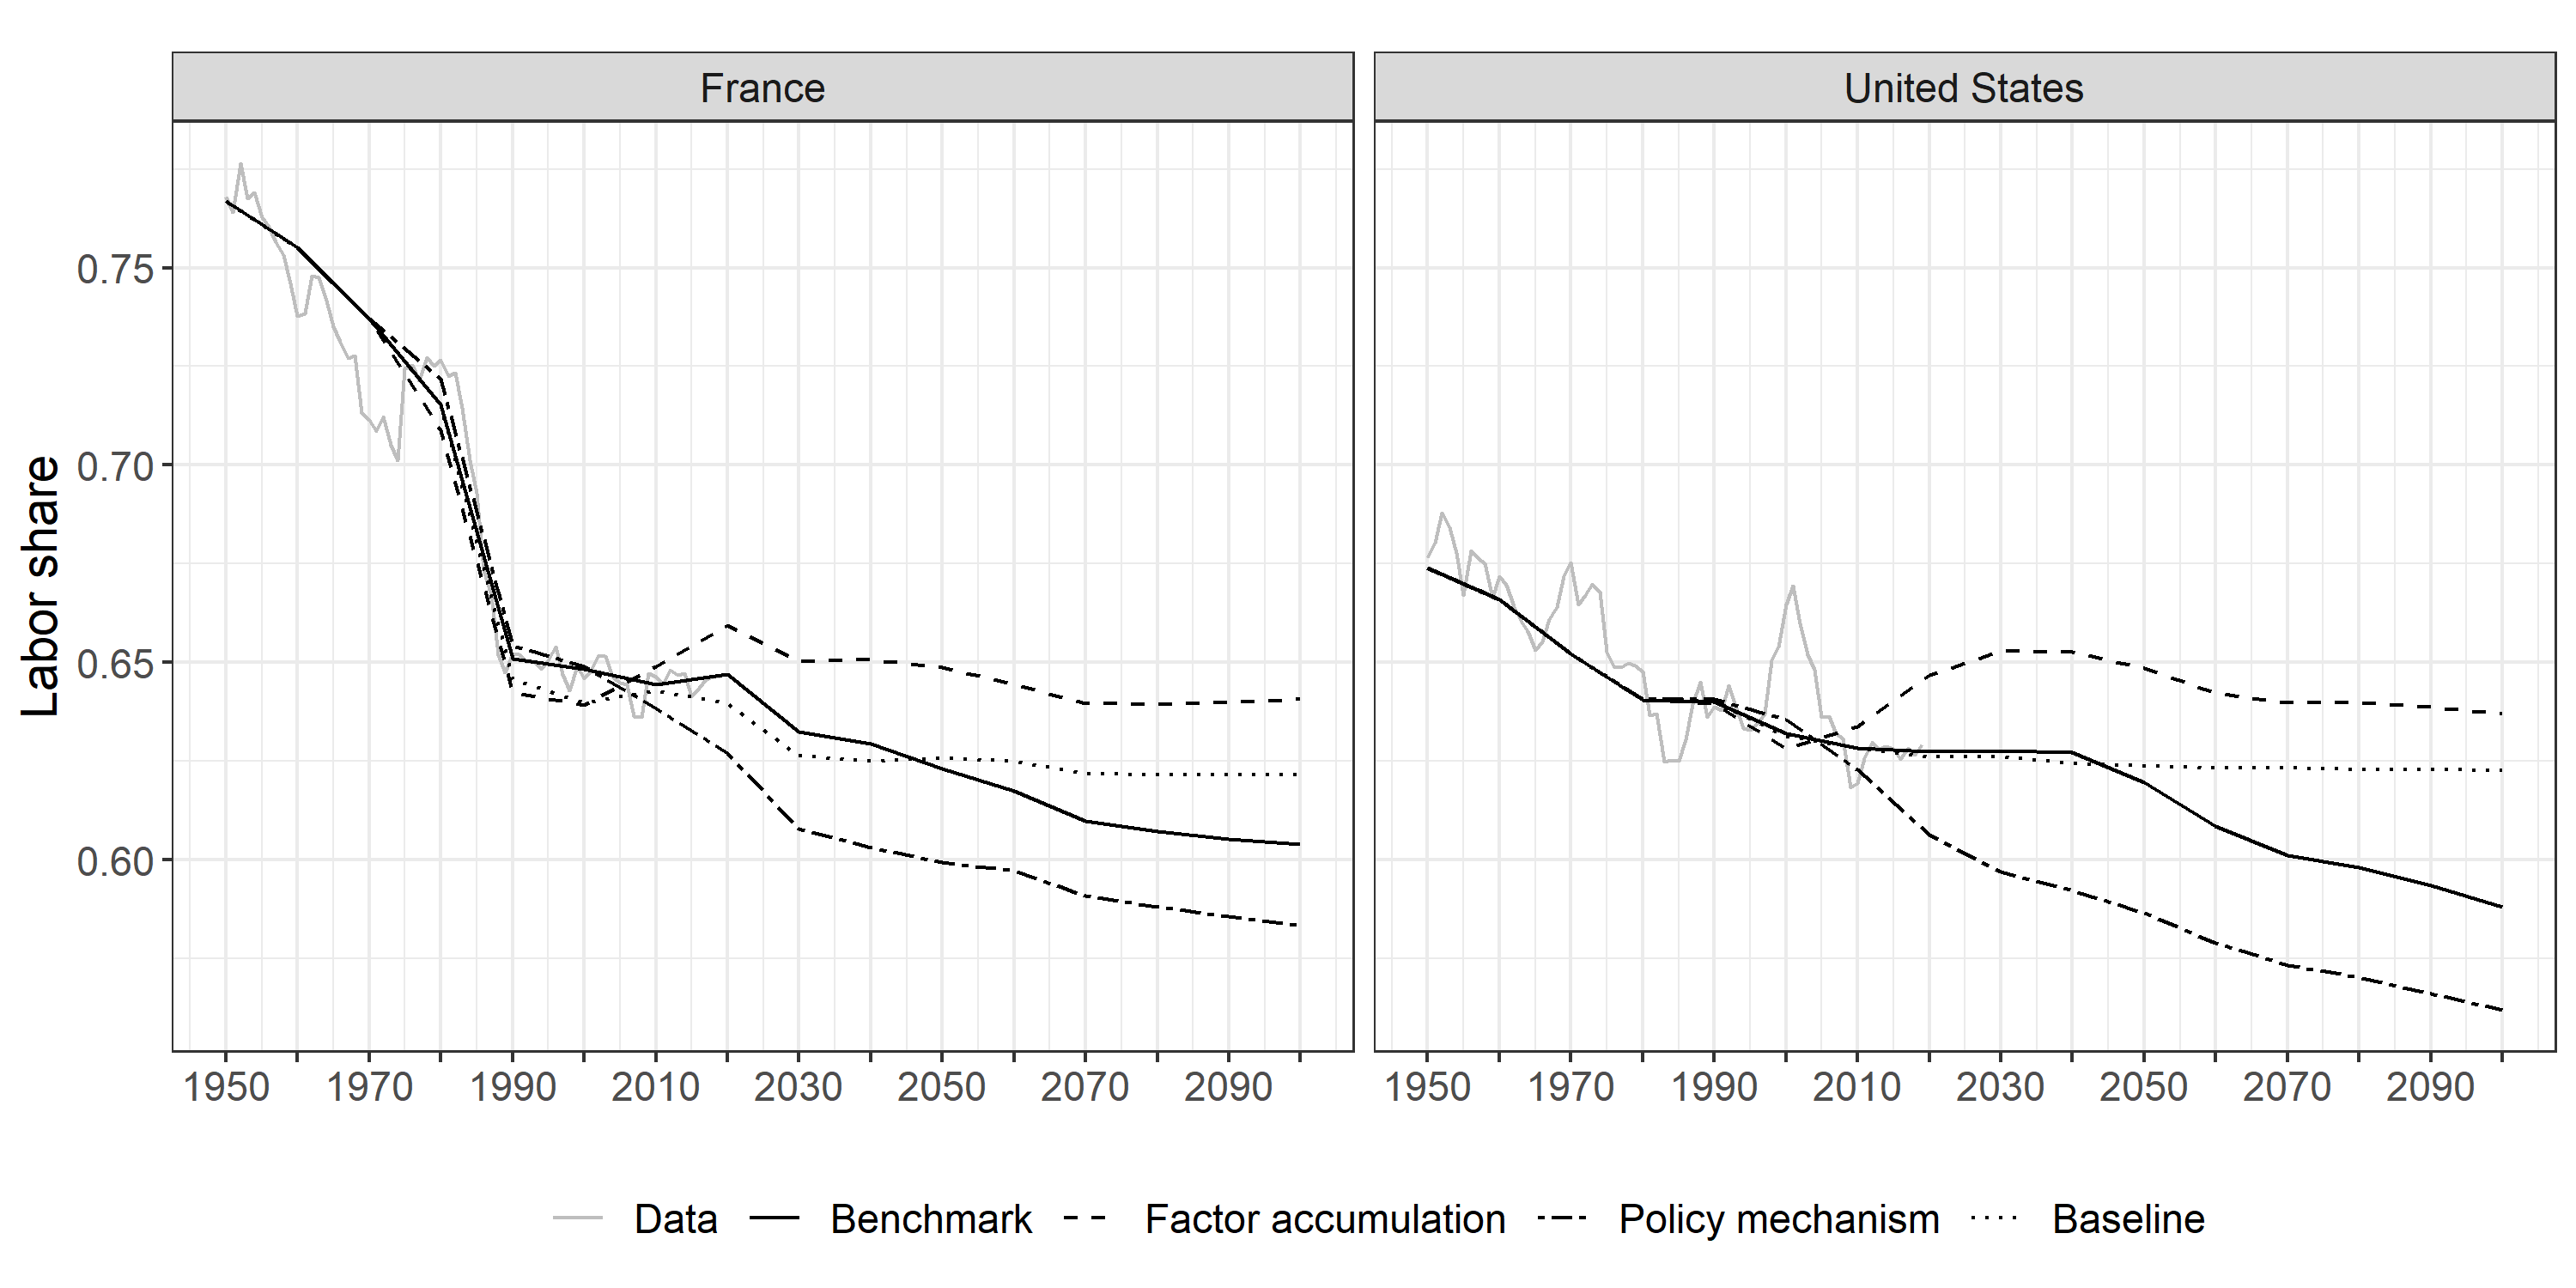
\includegraphics[width=1\linewidth]{chap1/graphic/quant-counter-channel.png}
	\vspace{-3em}
	\justify\singlespacing\footnotesize\textit{Notes:} The figure shows the counterfactual simulations of the channels of demographic changes on the labor share. 
	Labor share data are from the \href{https://www.rug.nl/ggdc/productivity/pwt/}{Penn World Table 9.1} with self-employed income as labor compensation.
	The benchmark labor share corresponds to the benchmark predictions of the model. The factor-accumulation simulation refers to the labor share of the counterfactual simulation in which the factor-accumulation channel is neutralized. The policy-mechanism simulation refers to the labor share of the counterfactual simulation in which the policy-mechanism channel is neutralized. The baseline labor share corresponds to the predictions when both channels are neutralized.
\end{figure}
From this figure, I derive the decomposition of the channels of demographic changes, see figure \ref{chap1-fig:quant-decomp-channel}.

\end{refsection}